\documentclass[11pt,letterpaper]{article}
\usepackage[utf8]{inputenc}
\usepackage[T1]{fontenc}
\usepackage[spanish,es-nodecimaldot]{babel}
\usepackage[margin=2.2cm]{geometry}
\usepackage{graphicx,booktabs,longtable,array,xcolor,hyperref,float,caption}
\usepackage[expansion=false]{microtype}
\hypersetup{colorlinks=true,linkcolor=blue!45!black,urlcolor=blue!55!black}
\graphicspath{{../../outputs/parte_3/05_mapas/}{../../outputs/parte_3/06_analisis/figuras/}}
\newcommand{\pregunta}[1]{\subsection{#1}}
\newcommand{\metodo}[1]{\paragraph{Método y variables.} #1}
\newcommand{\resultado}[1]{\paragraph{Resultado e interpretación.} #1}
\newcommand{\limite}[1]{\paragraph{Limitación.} #1}
\title{Parte 3: integración territorial de actividad textil,\\saneamiento e hidrografía en la cuenca del Alto Atoyac}
\author{Nuria Arroyo Bustamante\\173605\\Universidad de las Américas Puebla}
\date{2 de octubre de 2026}
\begin{document}
\maketitle
\begin{abstract}
Se construyó una base geoespacial común que integra 4,365 establecimientos del universo textil de la Parte 2, 22 clusters, 18 subnúcleos diagnósticos, 69 registros de plantas de tratamiento de aguas residuales (PTAR), 302 puntos de descarga, límites municipales y 12,161 segmentos de hidrografía superficial dentro de la cuenca. La integración preserva fuente, año y nivel de evidencia, y separa registros administrativos de inferencias por proximidad. No se encontraron geometrías recuperables de colectores. Los resultados permiten describir coincidencias territoriales, distancias y vacíos de información, pero no reconstruir todavía conexiones hidráulicas ni atribuir descargas a establecimientos.
\end{abstract}
\tableofcontents

\section{Objetivo y alcance}
El objetivo de la Parte 3 es homologar la información territorial de actividad textil con la infraestructura hídrica y de saneamiento disponible, de modo que análisis posteriores puedan estudiar conectividad, presión potencial, cobertura de tratamiento y sitios de monitoreo. La unidad de integración es espacial, pero una distancia corta no se interpreta como conexión. Tampoco se evalúa causalidad de contaminación ni suficiencia del tratamiento.

\section{Fuentes, temporalidad y modelo de integración}
Los establecimientos, clusters y subnúcleos provienen de la solución congelada de Parte 2. Las PTAR y descargas proceden del Censo Nacional de Gobiernos Municipales y Demarcaciones Territoriales 2021 de INEGI, distribuido en 2023, y de una compilación manual con registros de 2021--2022. La hidrografía corresponde a la red RH18 escala 1:50,000. Los límites de cuenca y municipios provienen de los insumos territoriales organizados previamente. El reporte y proyecto QGIS de Lesly se usaron como evidencia documental y estructural.

Todas las capas métricas se homologaron en EPSG:32614. Se asignaron identificadores internos estables, sin sustituir los identificadores de origen. Los niveles de evidencia son: A, fuente explícita u oficial; B, consistencia entre fuentes; C, plausibilidad espacial o documental parcial; y D, información desconocida o insuficiente.

La Figura~\ref{fig:contexto} presenta el ámbito común. La red azul incluye afluentes y no solamente el cauce principal.
\begin{figure}[H]\centering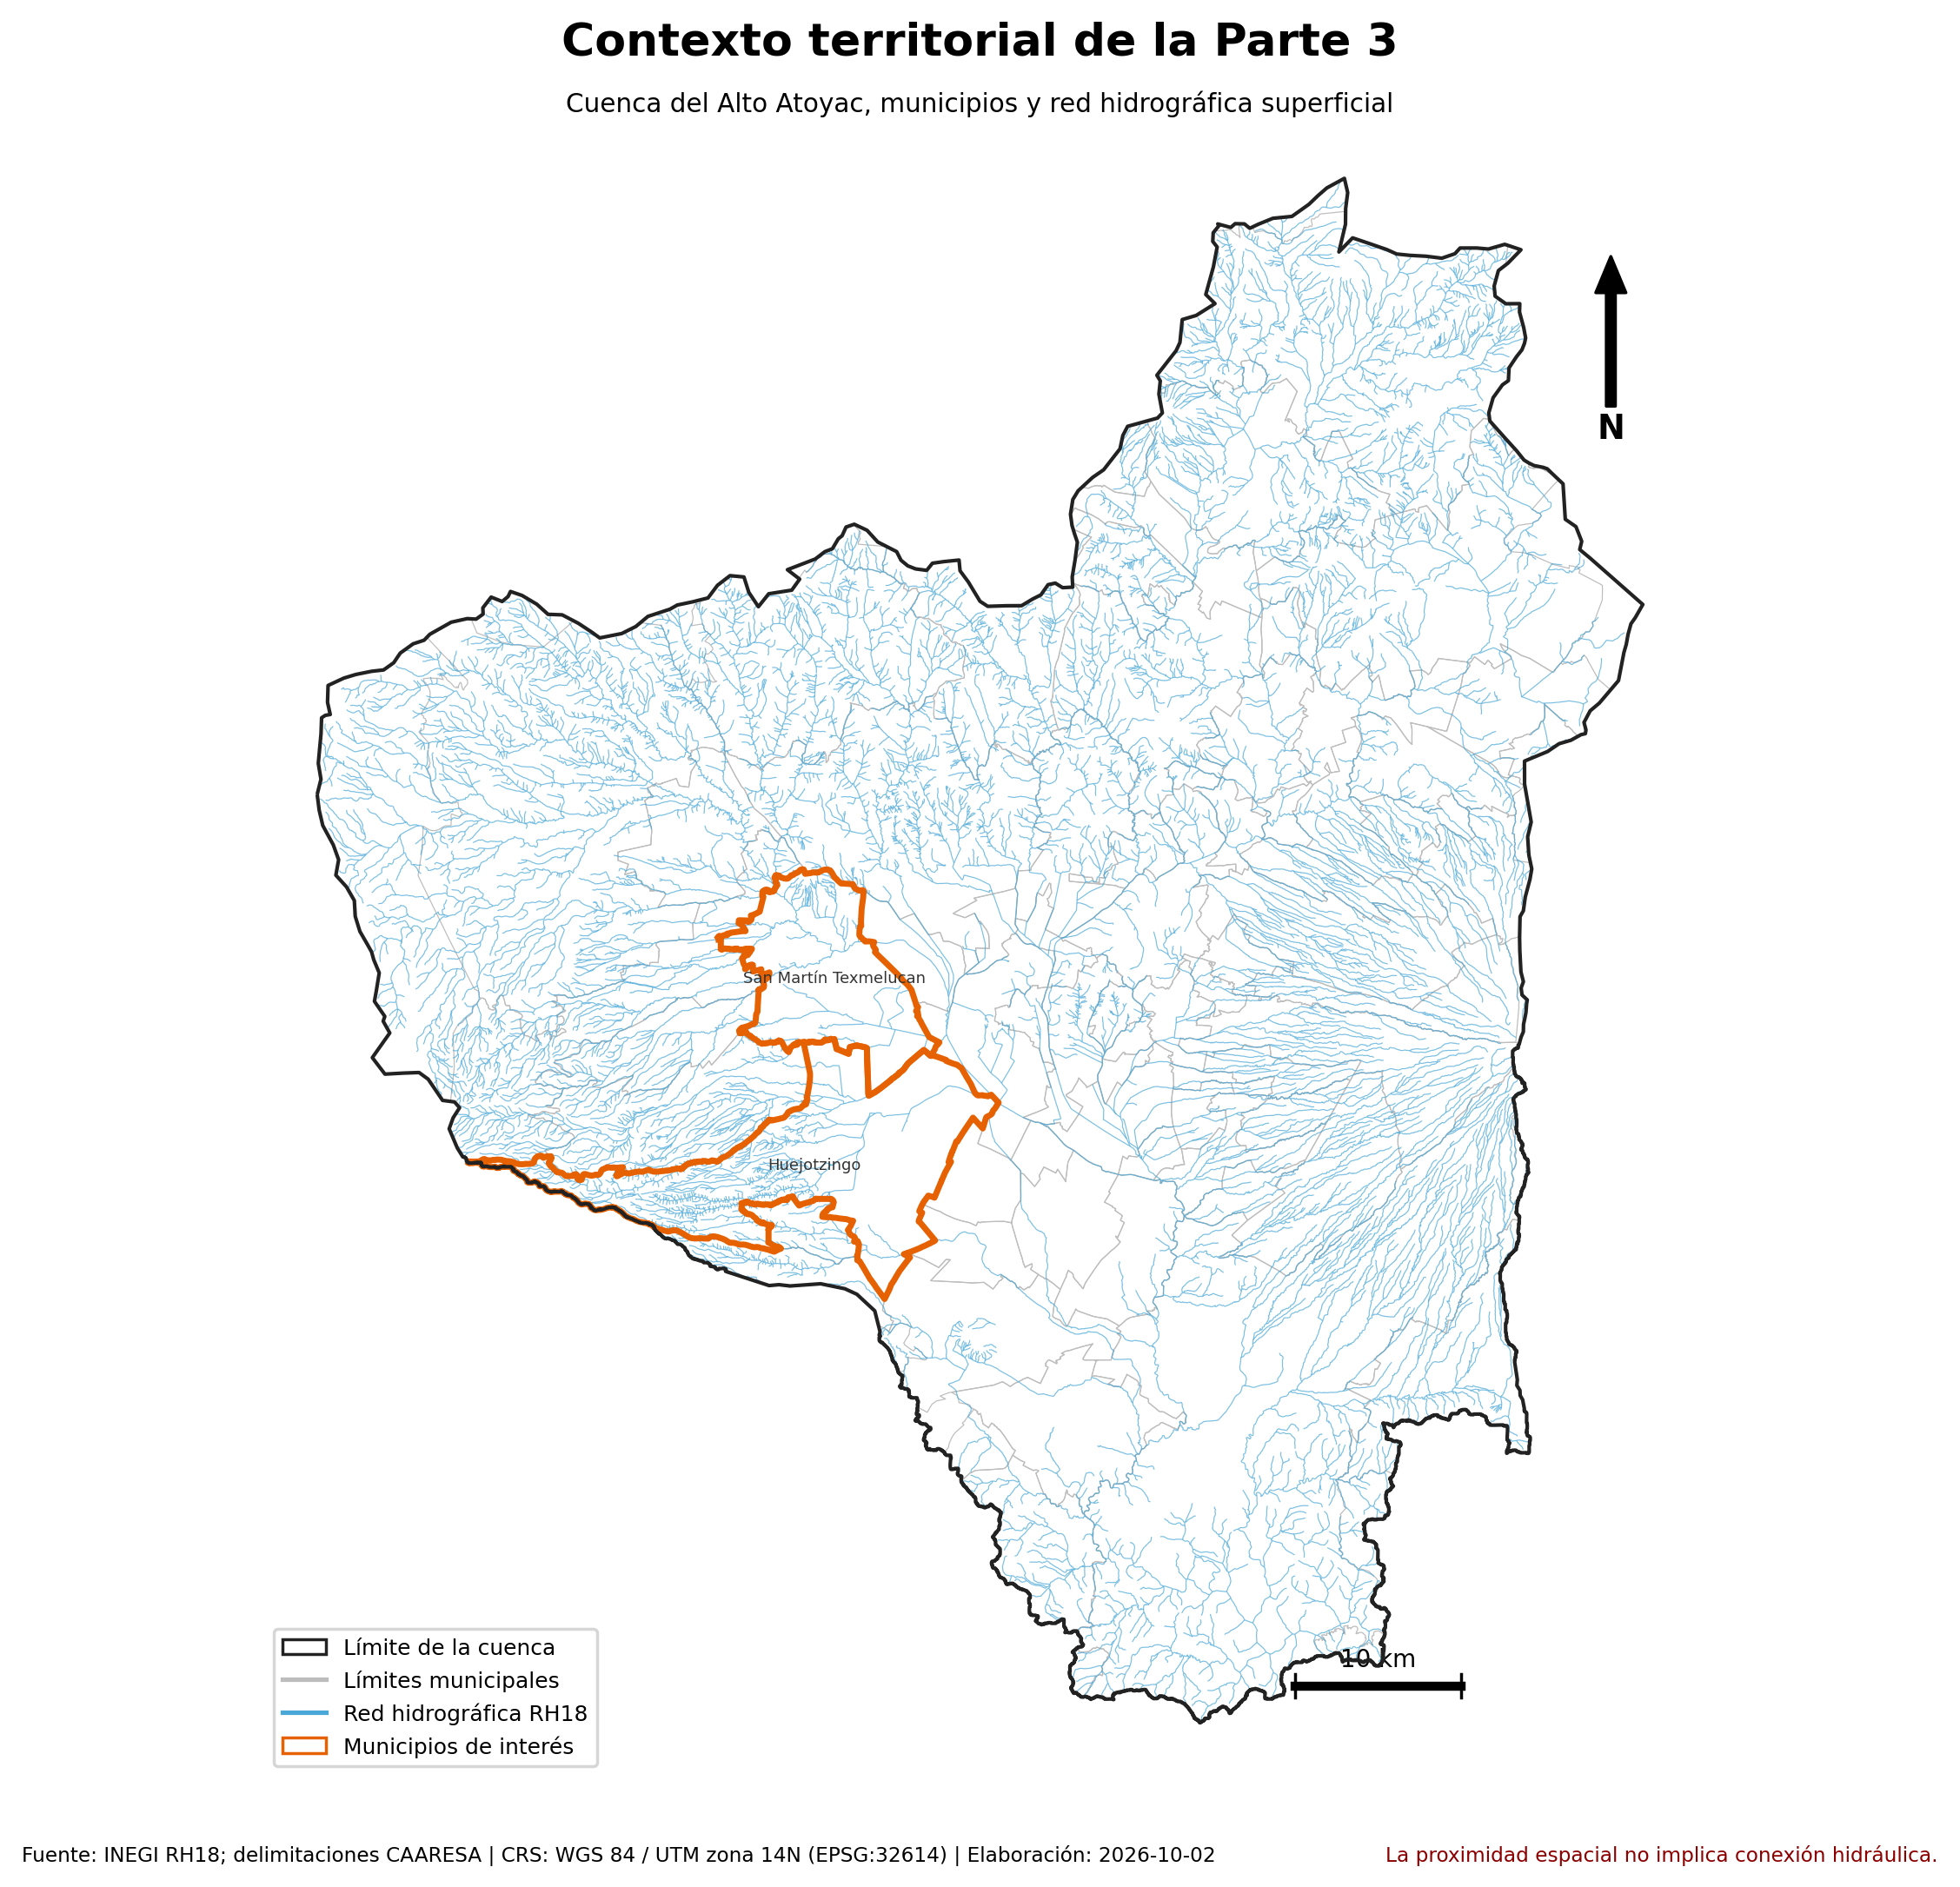
\includegraphics[width=.9\textwidth]{01_contexto_territorial.png}\caption{Contexto territorial, límites municipales e hidrografía superficial. Huejotzingo y San Martín Texmelucan se resaltan como municipios de interés.}\label{fig:contexto}\end{figure}

\section{Inventario integrado y diferencias semánticas}
La base contiene 65 registros de PTAR de INEGI y cuatro registros manuales de PTAR. Un quinto registro de la compilación, Global Denim, declara explícitamente ser una descarga industrial y fue integrado en \emph{descargas}, no en \emph{PTAR}. Una coincidencia exacta de nombre, municipio y coordenadas fue marcada como posible duplicado entre fuentes, pero no se fusionó. Por tanto, los 69 registros no equivalen necesariamente a 69 plantas físicamente distintas.

INEGI registra 301 puntos como descarga sin permitir, en el recorte disponible, distinguir de manera consistente entre municipal e industrial. El registro manual adicional conserva su tipo industrial. La red RH18 representa drenaje natural e hidrografía superficial; no es una red de alcantarillado.

\section{PTAR, descargas y colectores}
La Figura~\ref{fig:ptar} muestra que las PTAR registradas se distribuyen en buena parte de la cuenca, mientras que los cuatro registros manuales se concentran en los municipios de interés. Registro no significa operación actual, área de servicio o capacidad disponible.
\begin{figure}[H]\centering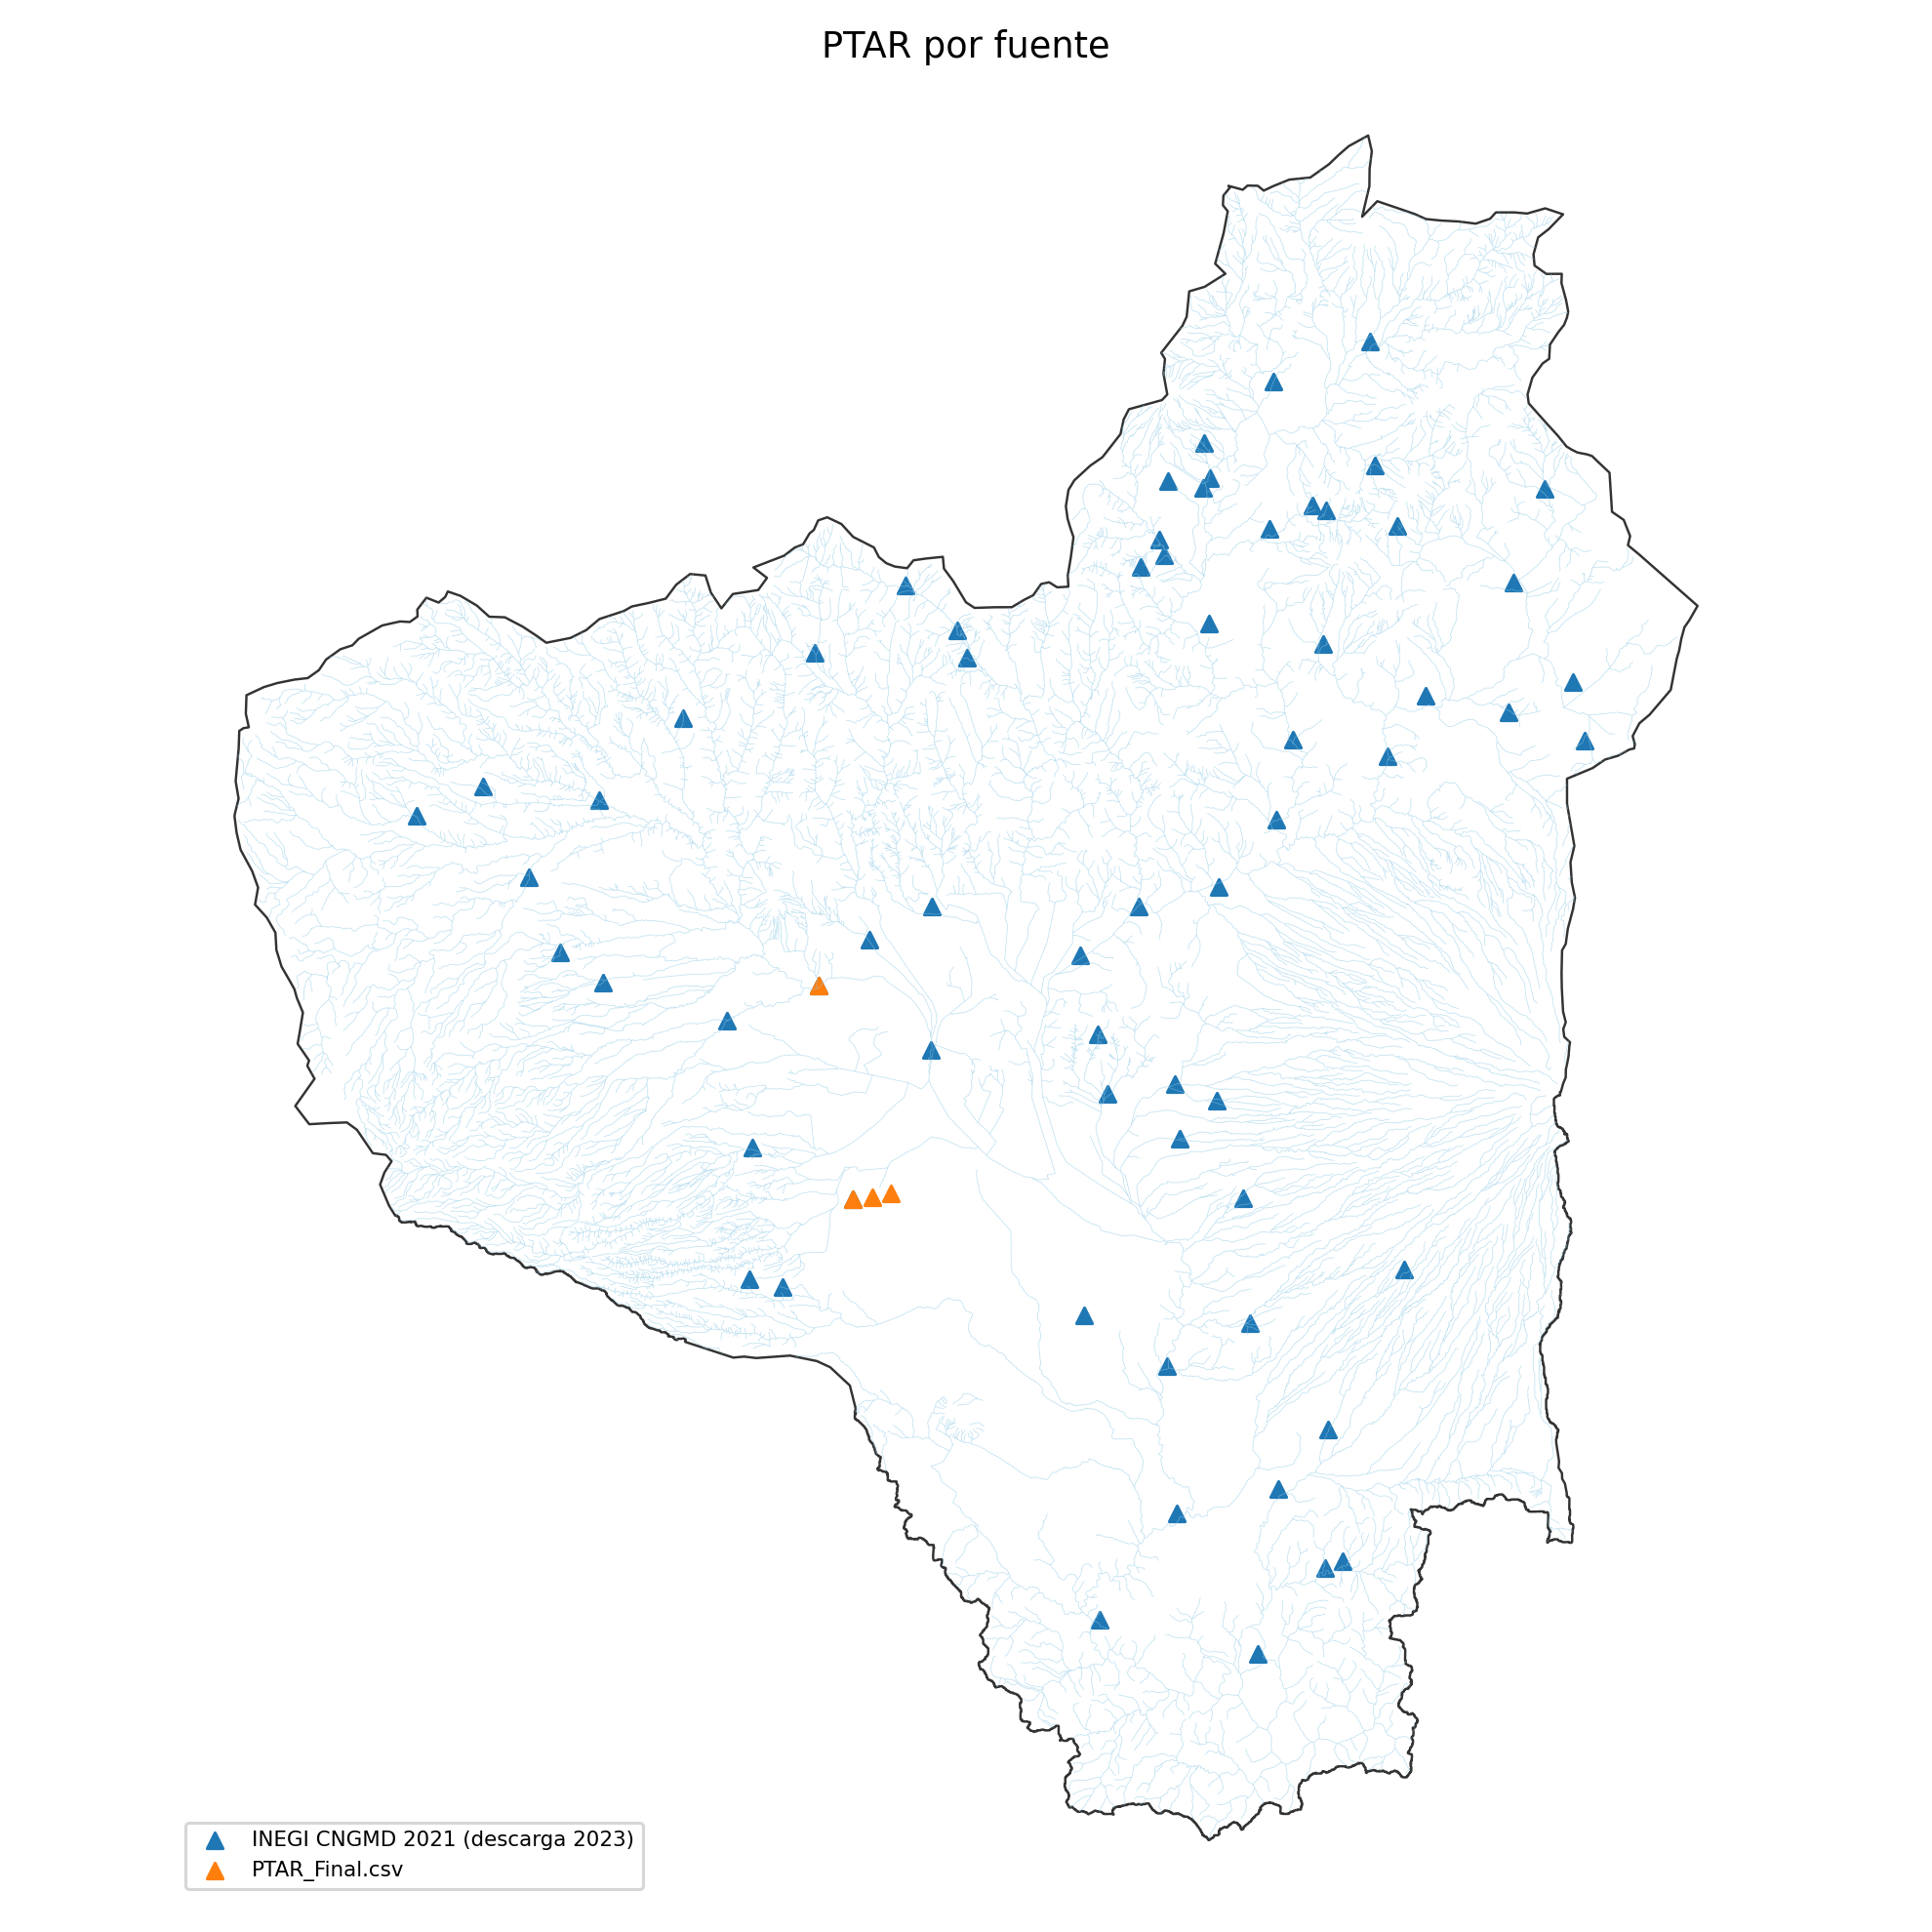
\includegraphics[width=.86\textwidth]{03_ptar_tipo_fuente.png}\caption{PTAR diferenciadas por fuente y temporalidad.}\label{fig:ptar}\end{figure}

La Figura~\ref{fig:descargas} muestra 302 descargas y su relación visual con la red superficial. El mapa permite observar proximidades, no concluir el cauce receptor efectivo salvo donde éste figure como atributo declarado.
\begin{figure}[H]\centering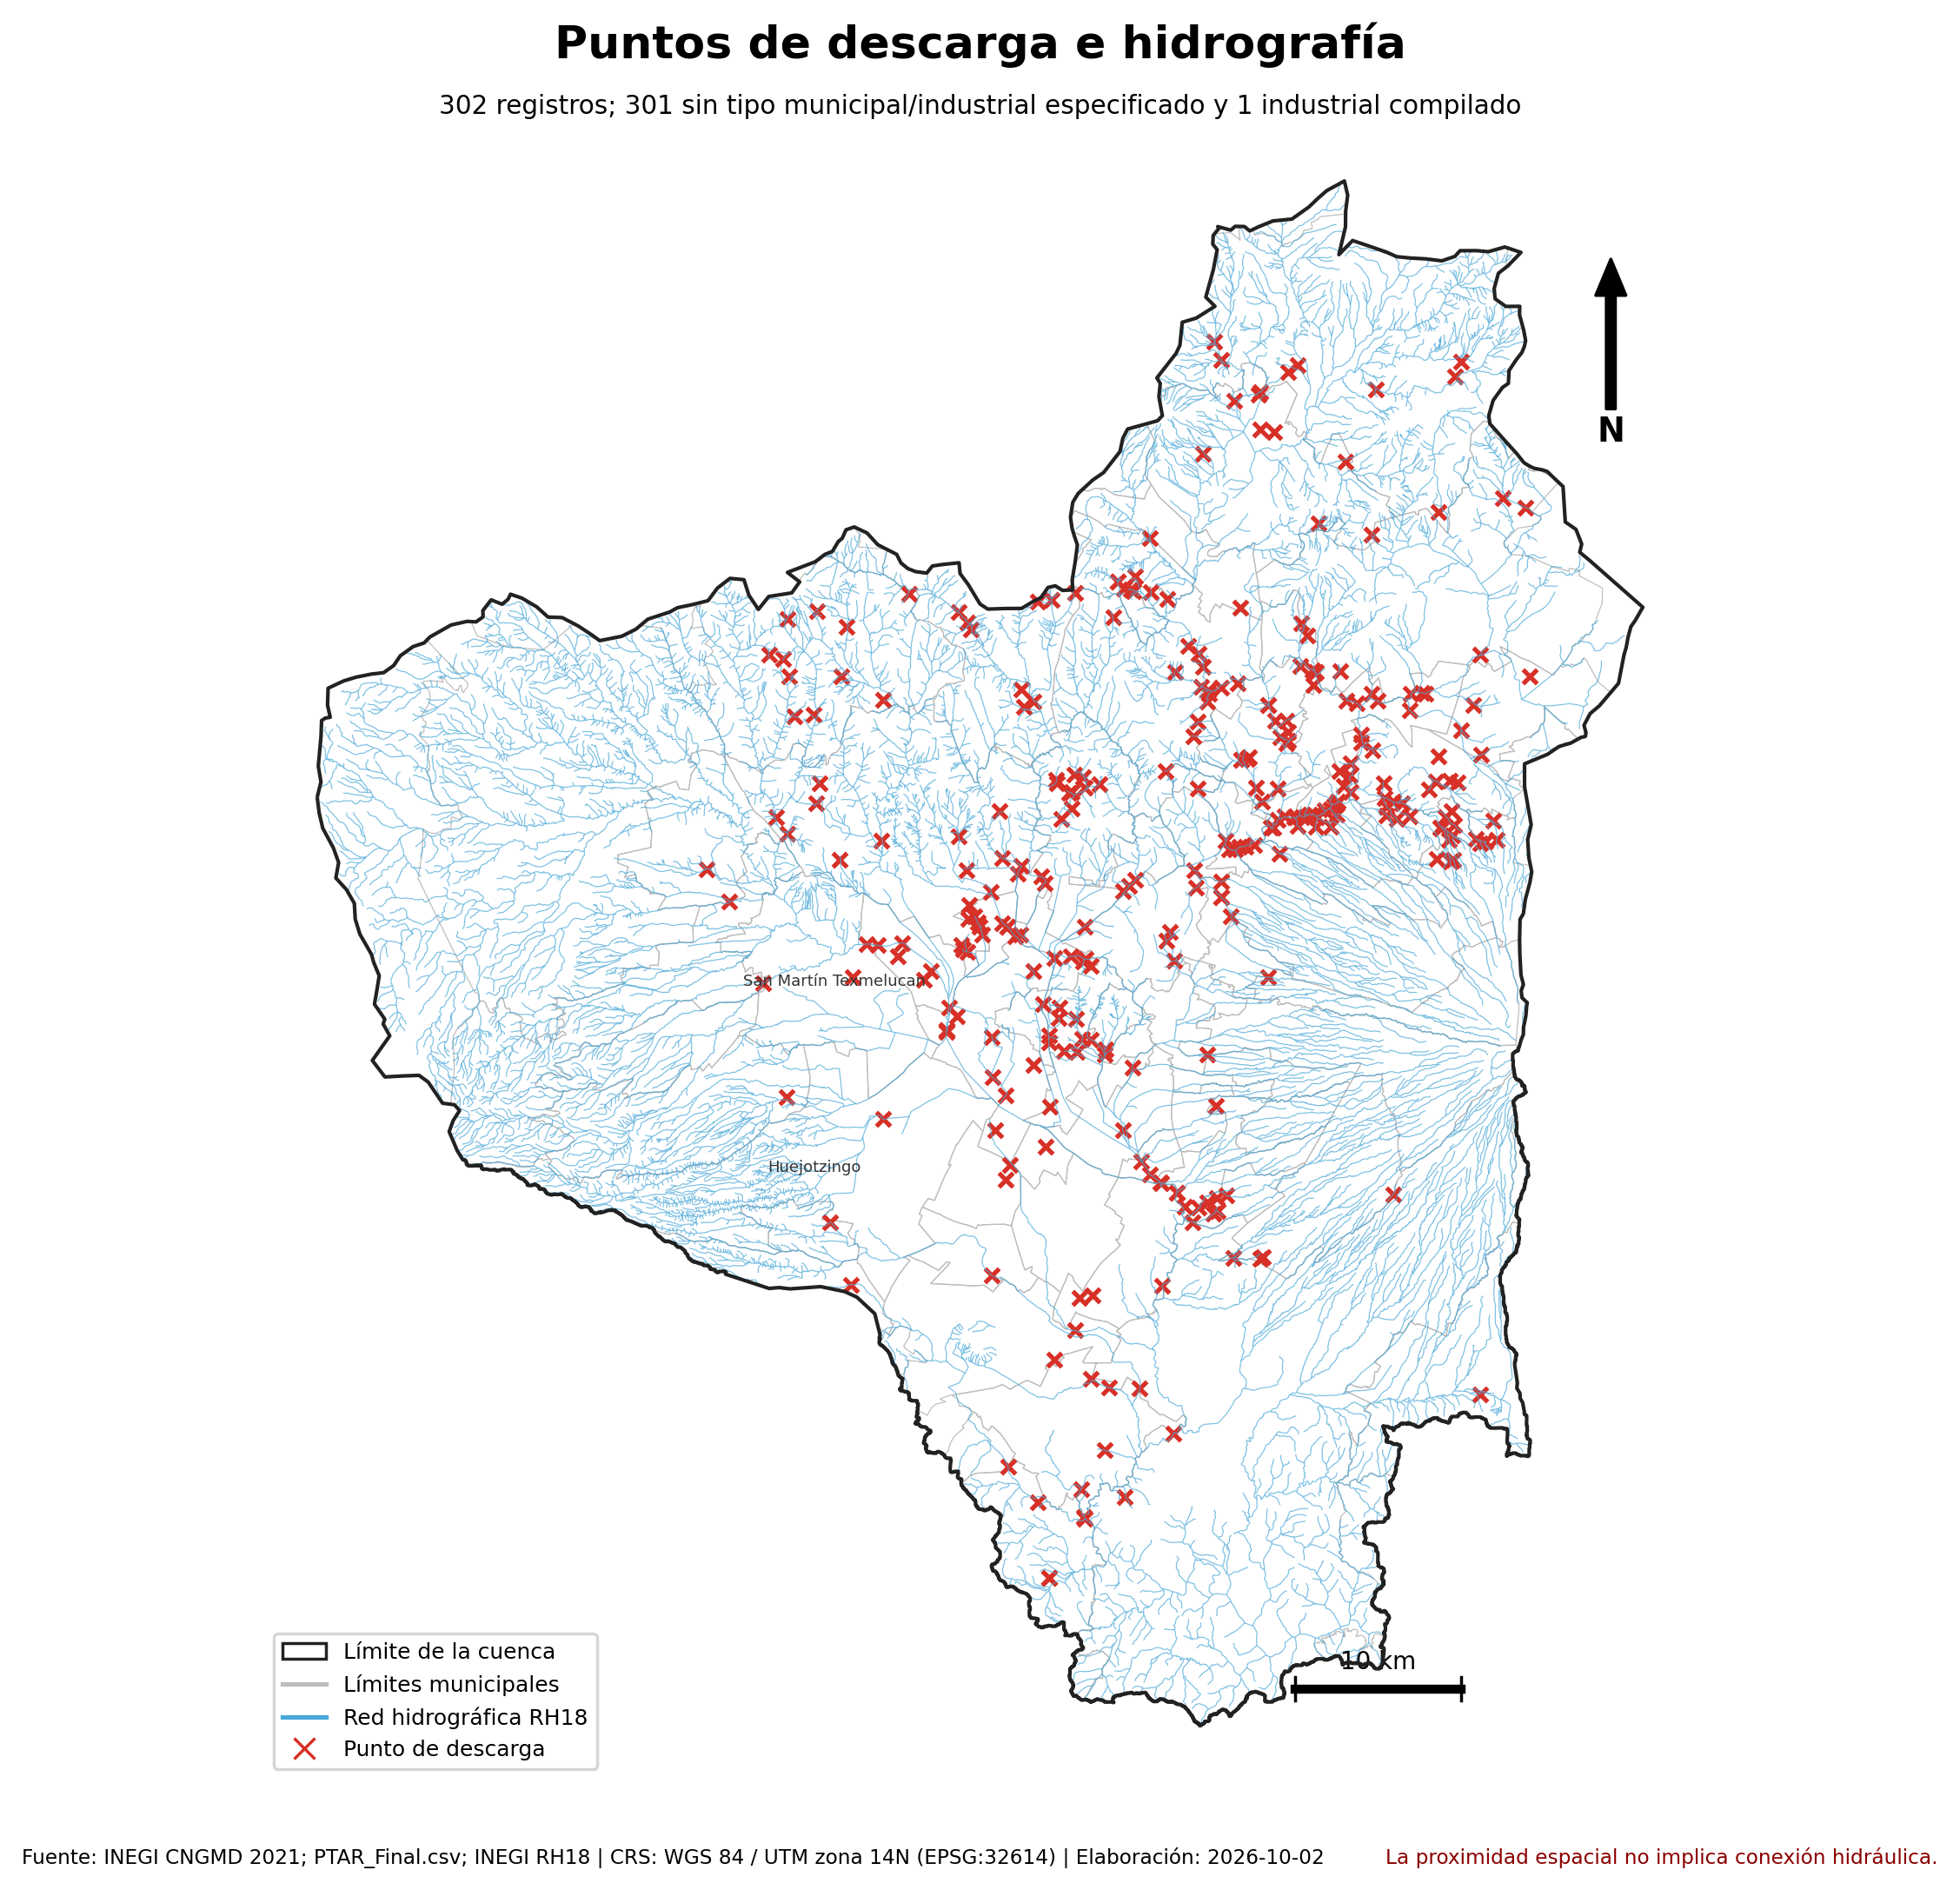
\includegraphics[width=.86\textwidth]{04_descargas_hidrografia.png}\caption{Puntos de descarga e hidrografía superficial disponible.}\label{fig:descargas}\end{figure}

No existe una capa recuperable de colectores. Los nombres \texttt{Camino\_contenedores\_SMT} y \texttt{Camino\_contenedores\_huejotzingo} aparecen como nodos huérfanos en el proyecto QGIS. La Figura~\ref{fig:colectores} comunica este vacío y evita representar líneas propuestas como infraestructura existente.
\begin{figure}[H]\centering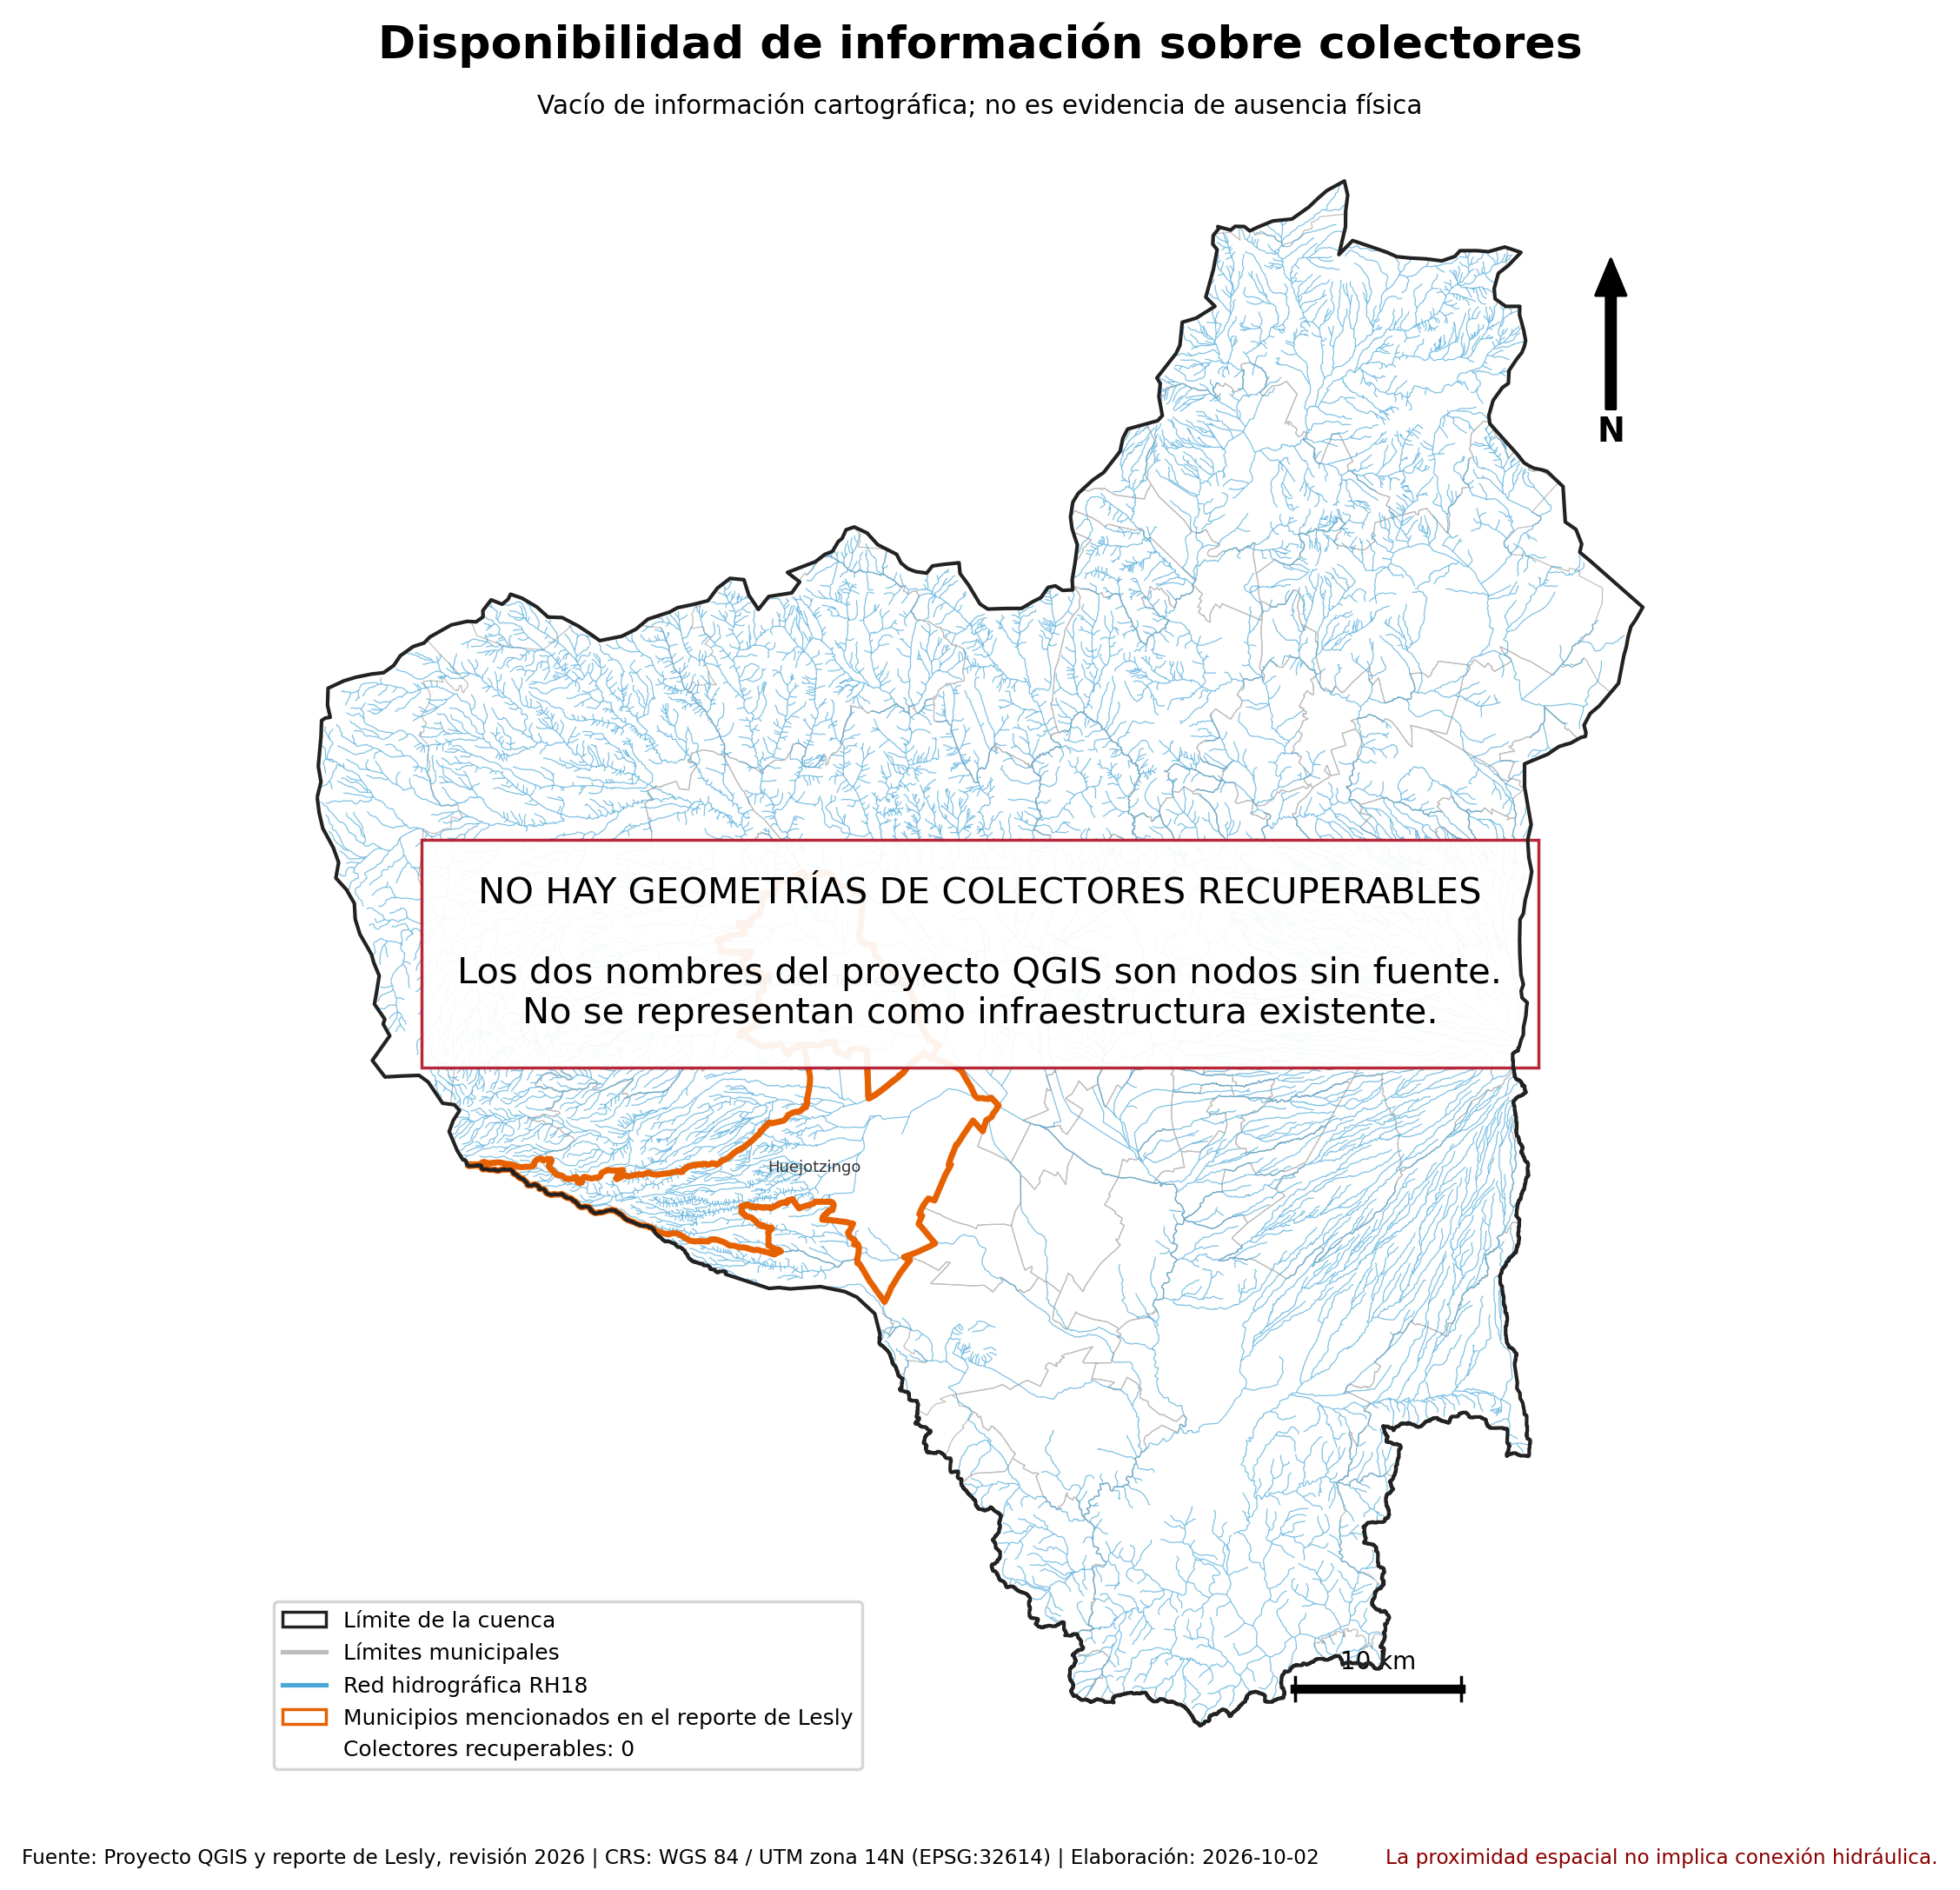
\includegraphics[width=.86\textwidth]{05_disponibilidad_colectores.png}\caption{Disponibilidad de evidencia geográfica sobre colectores. La ausencia de geometrías no demuestra ausencia física de infraestructura.}\label{fig:colectores}\end{figure}

\section{Integración con los resultados de Parte 2}
Se conservaron los 4,365 establecimientos, los 22 clusters de la solución principal y los 18 subnúcleos exploratorios del cluster 20. Los establecimientos incluyen SCIAN, señales de proceso húmedo o seco, relevancia ambiental, probabilidad, persistencia y resultado espacial. Los 355 puntos fuera del límite estricto se mantienen como contexto de borde, pero la cartografía se encuadra en la cuenca.
\begin{figure}[H]\centering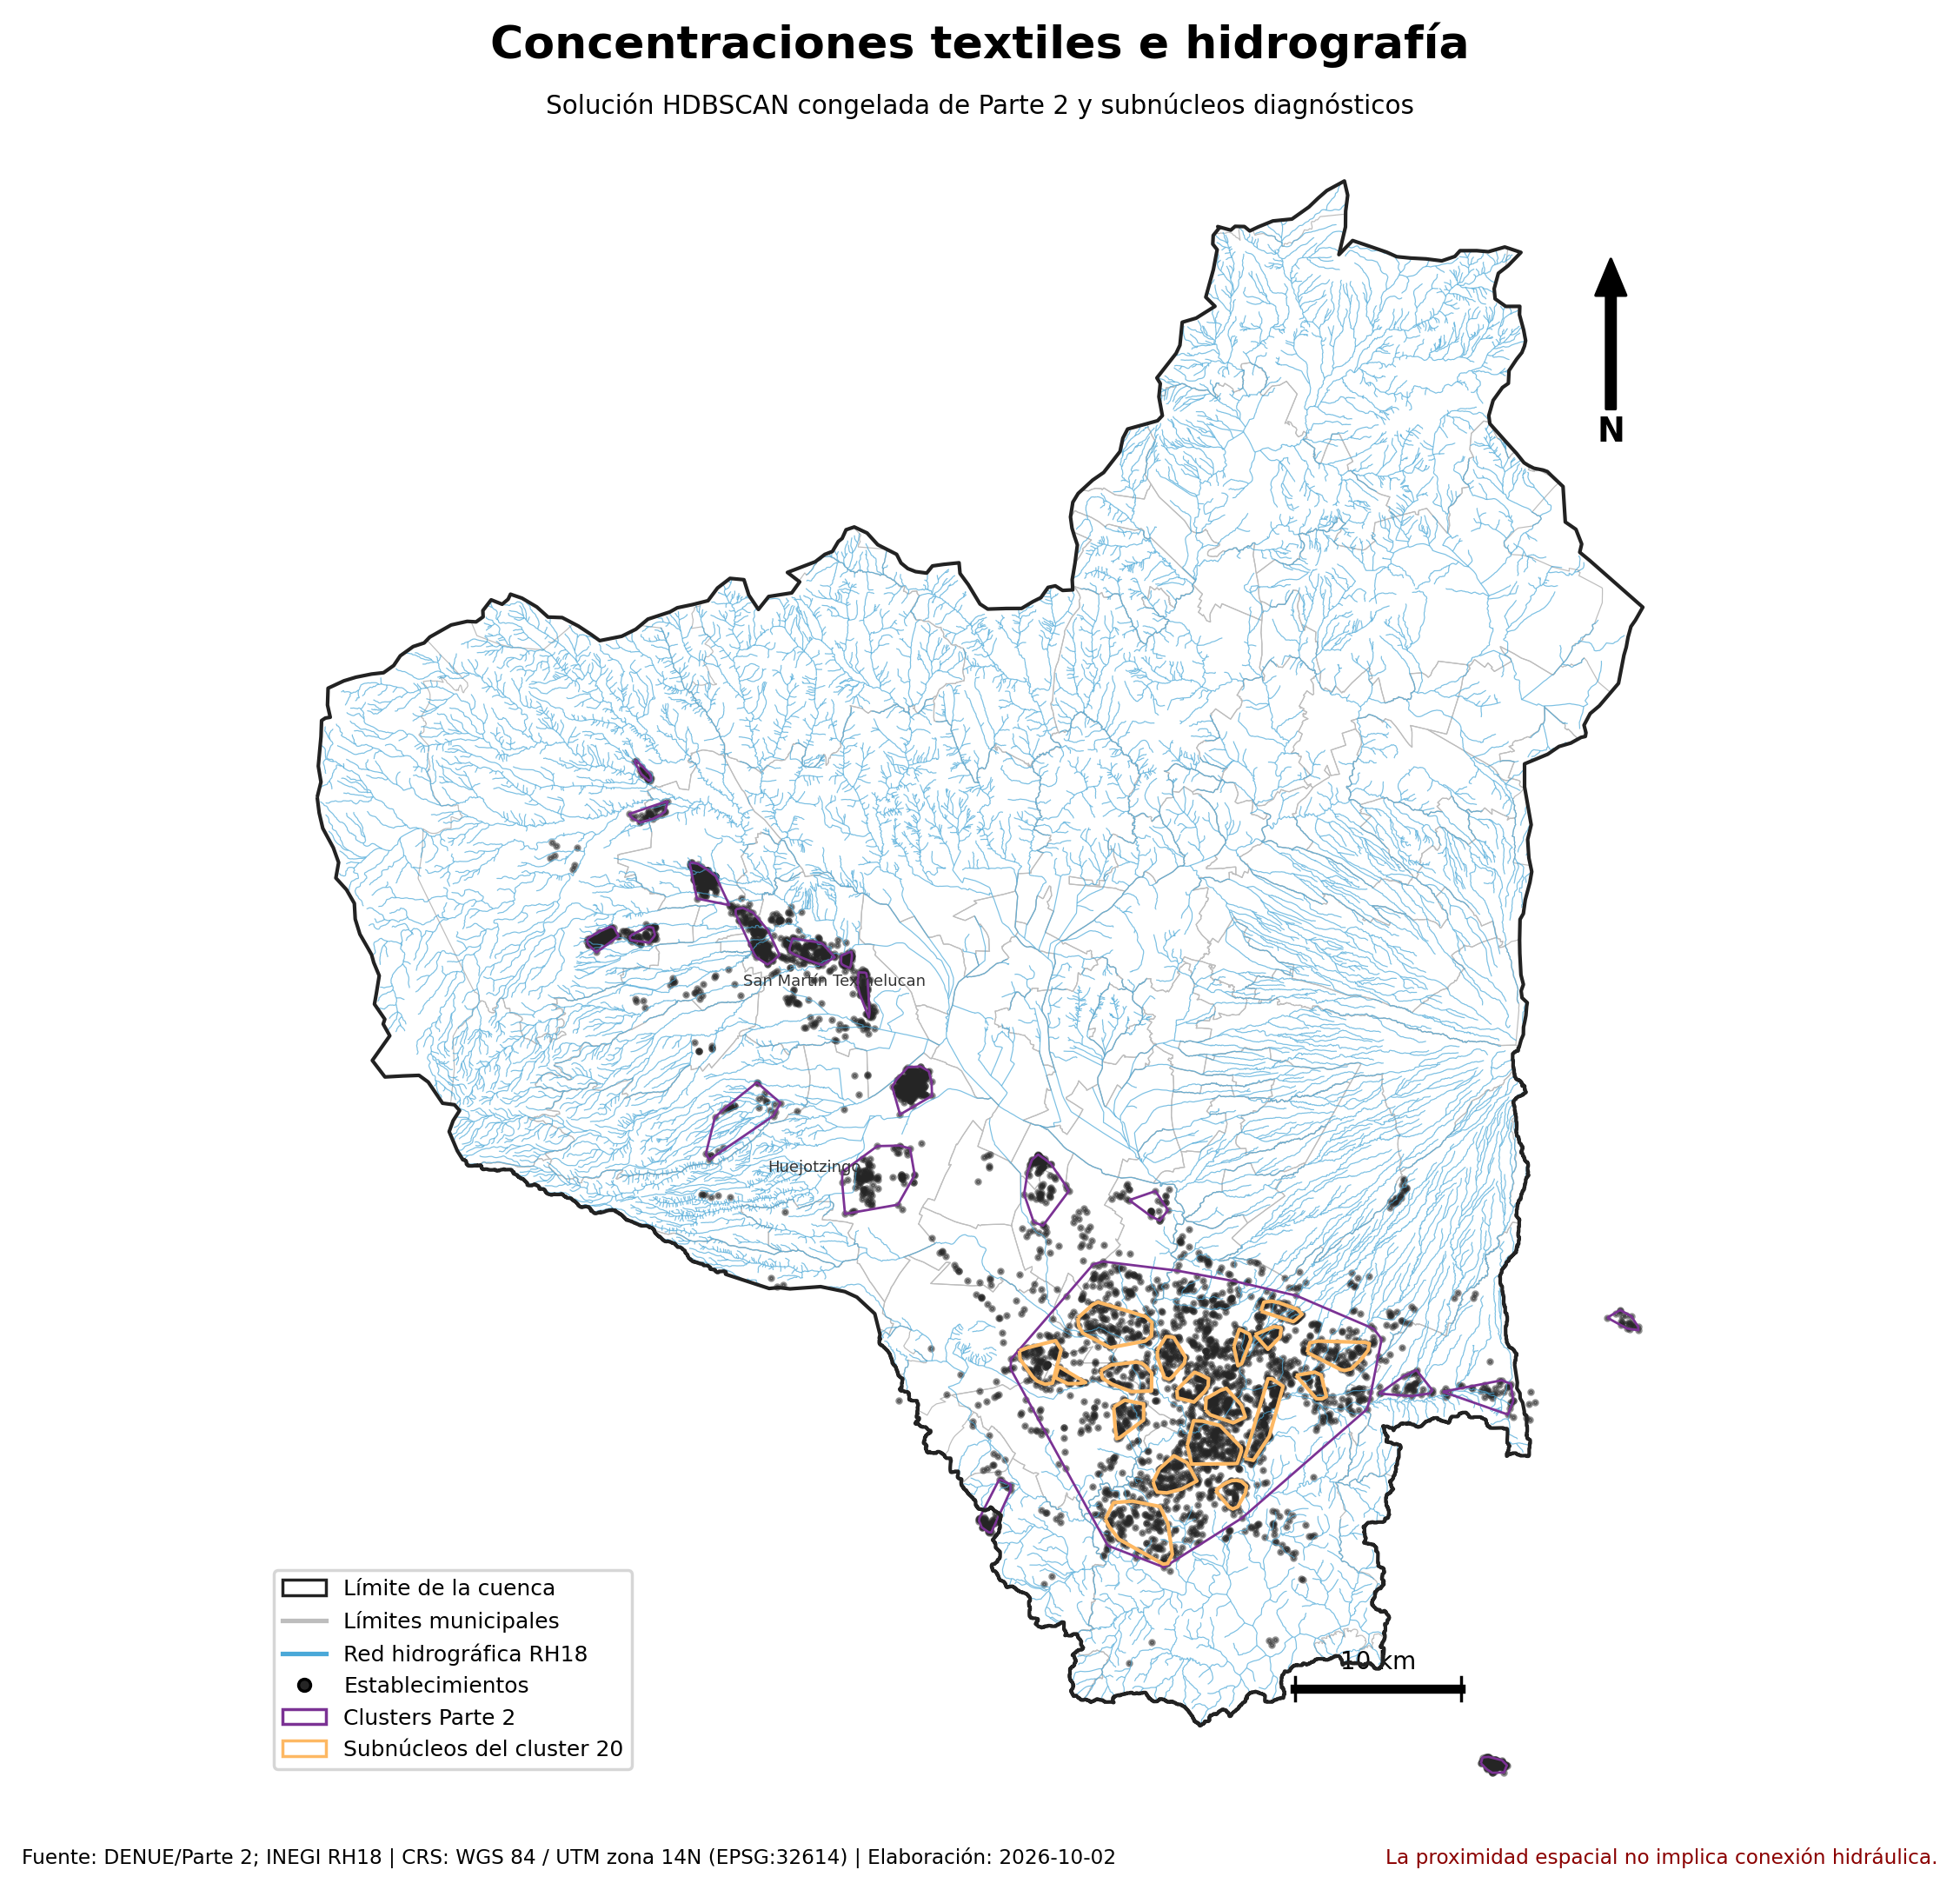
\includegraphics[width=.9\textwidth]{02_establecimientos_clusters_hidrografia.png}\caption{Concentraciones textiles, clusters, subnúcleos e hidrografía. Los subnúcleos son diagnósticos internos y no una nueva partición regional.}\label{fig:textil}\end{figure}

\section{Preguntas de investigación y resultados exploratorios}
\pregunta{P1. ¿Dónde coincide la concentración textil con infraestructura disponible?}
\metodo{Se superpusieron establecimientos, subnúcleos, PTAR y descargas en EPSG:32614; los colectores se mantuvieron como capa vacía.}
\resultado{La coincidencia se observa principalmente alrededor de subnúcleos que también presentan descargas y cauces próximos. La integración general de la Figura~\ref{fig:integracion} permite localizar estas coincidencias sin atribuir rutas.}
\limite{La superposición no demuestra que los establecimientos descarguen en esos puntos o sean atendidos por las PTAR cercanas.}
\begin{figure}[H]\centering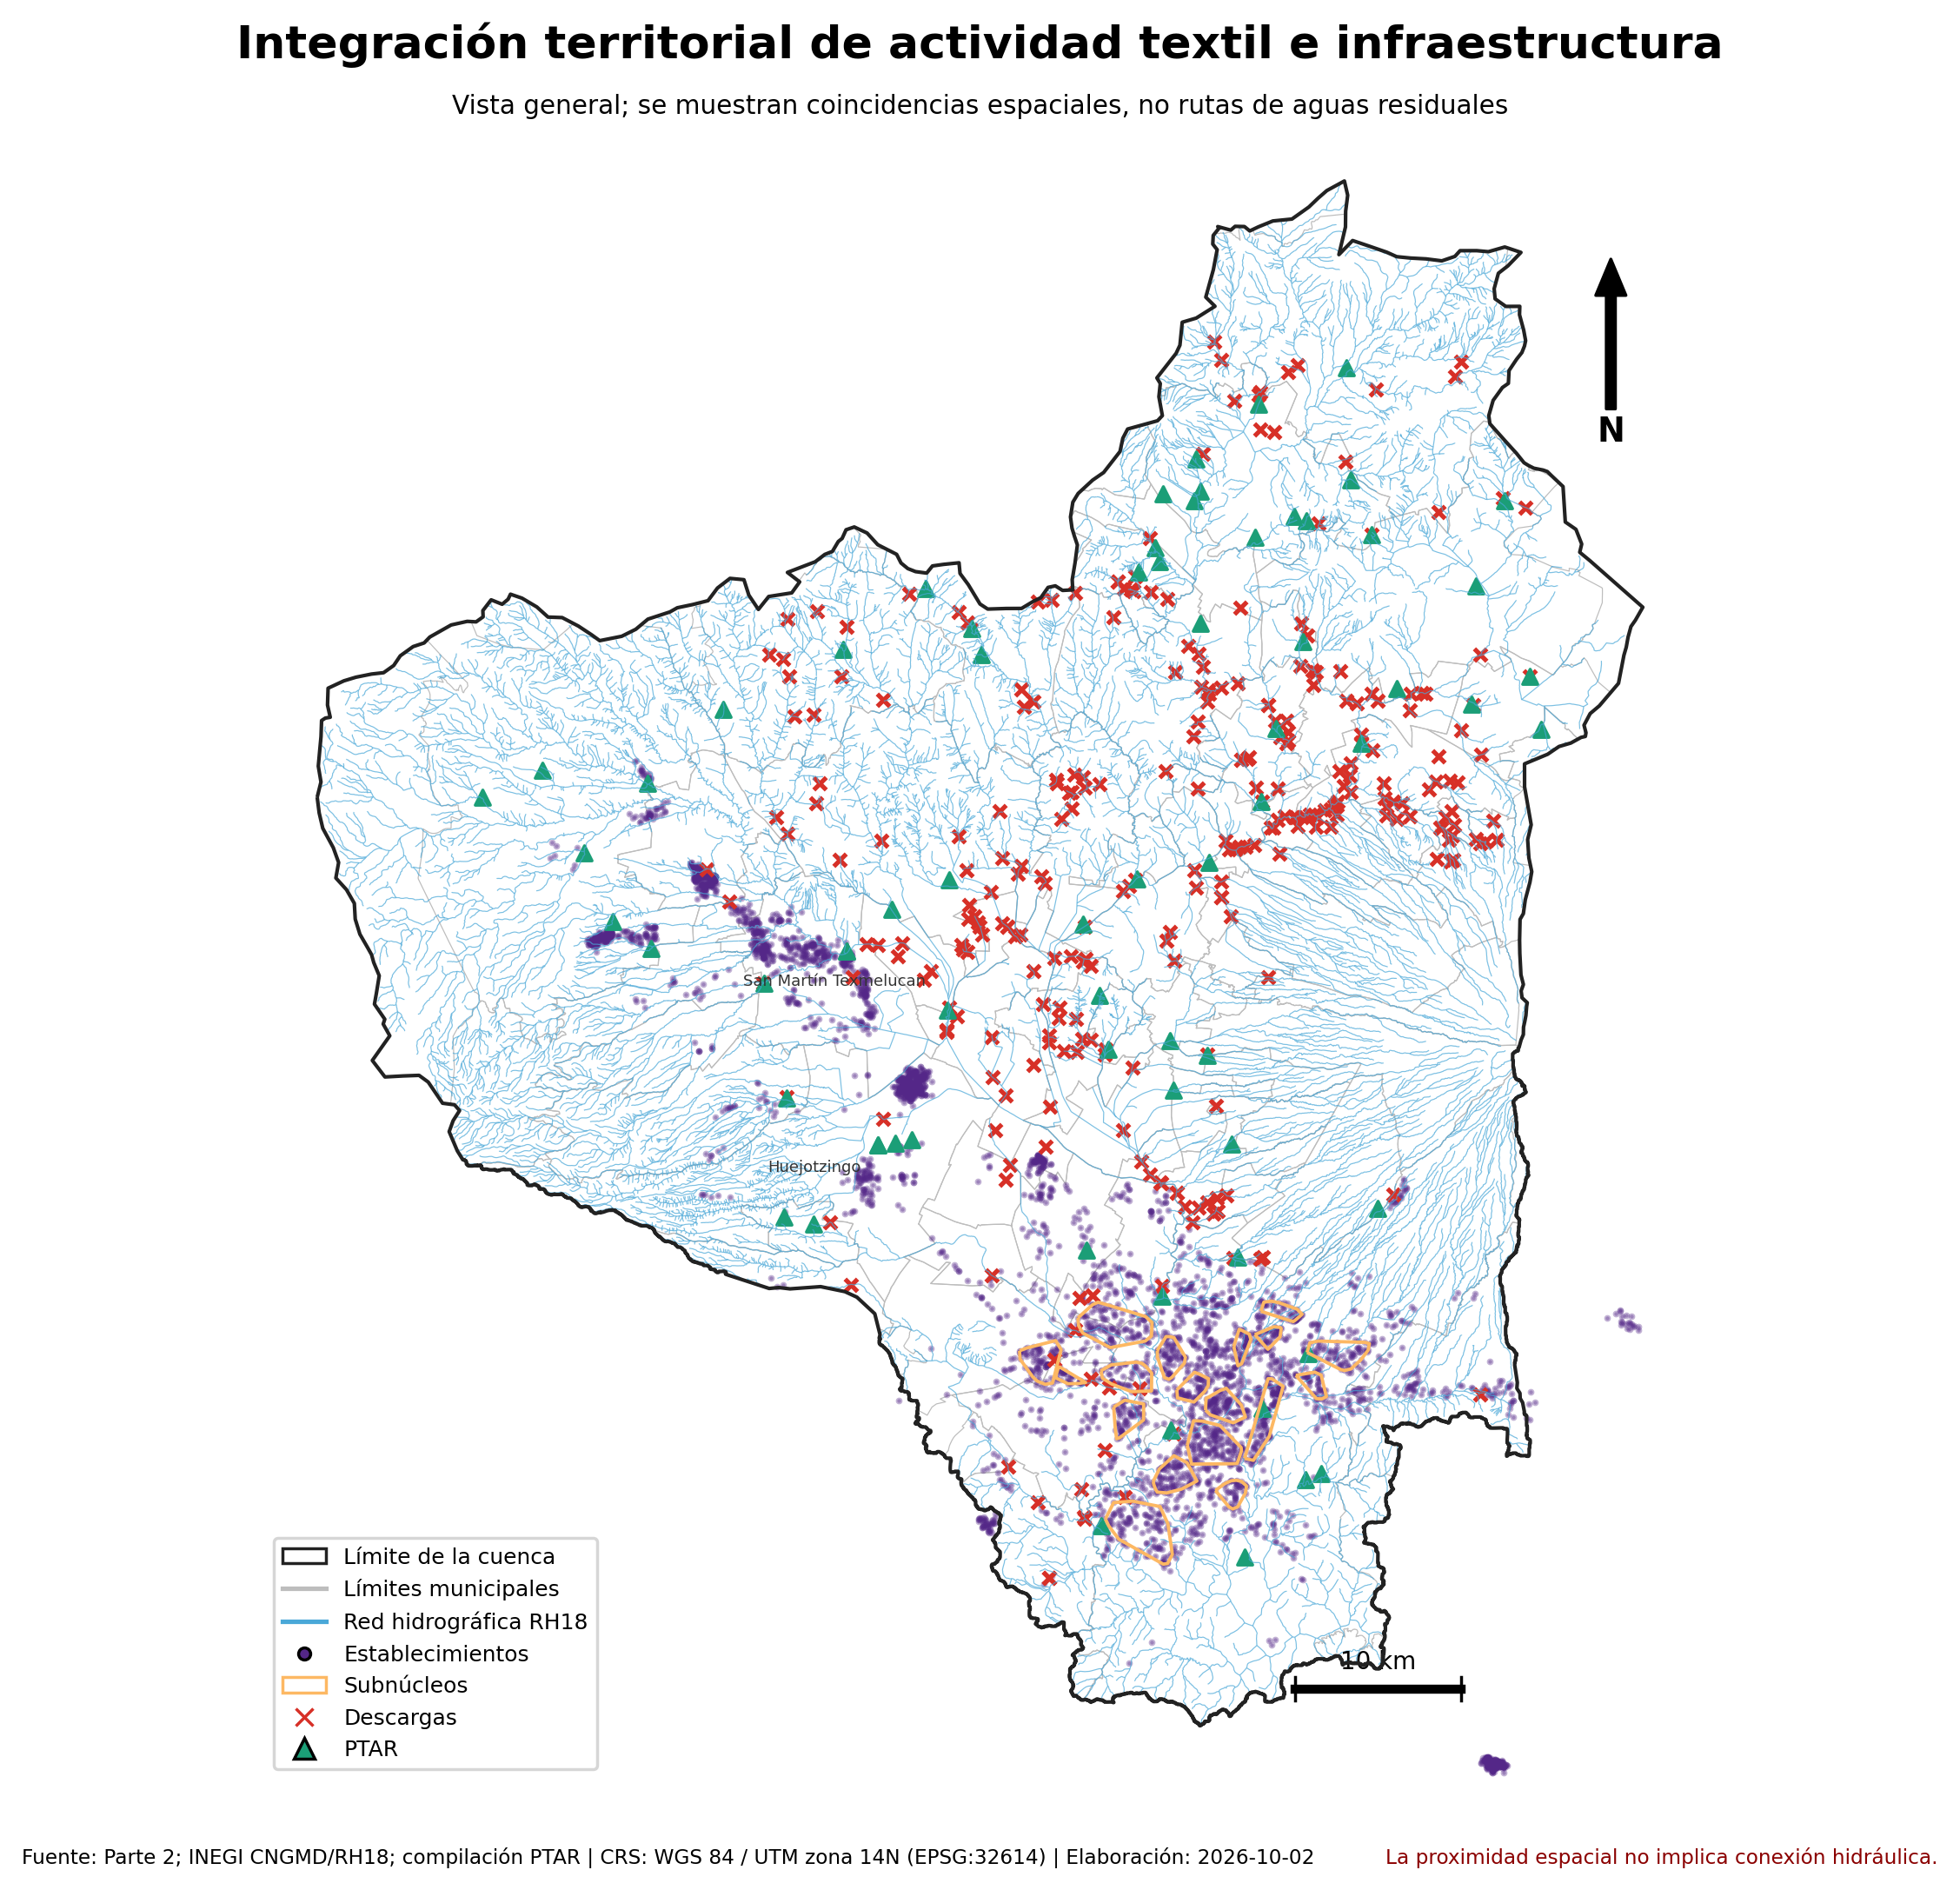
\includegraphics[width=.9\textwidth]{06_integracion_general.png}\caption{Integración territorial general. Los símbolos representan coexistencia espacial, no conexiones.}\label{fig:integracion}\end{figure}

\pregunta{P2. ¿Qué subnúcleos presentan mayor proximidad a infraestructura?}
\metodo{Para cada envolvente se calcularon establecimientos, relevancia alta/media, distancia mínima a descarga, PTAR e hidrografía, descargas a 1 km y PTAR a 5 km.}
\resultado{SUB\_01 y SUB\_02 intersectan geométricamente al menos una descarga; SUB\_04 y SUB\_05 están a 283 y 310 m de la descarga más próxima. SUB\_04 tiene tres PTAR a 5 km y la más próxima a 421 m; SUB\_05 tiene dos y la más próxima a 1,562 m. SUB\_00 queda a 37 m de la red hidrográfica, pero sin PTAR a 5 km. Las dimensiones se presentan por separado y no forman un ranking.}
\limite{No hay distancias a colectores porque no existe geometría fuente. Distancia cero puede indicar intersección con la envolvente, no coincidencia con cada establecimiento.}

\pregunta{P3. ¿Dónde hay menor información conocida sobre saneamiento?}
\metodo{Se marcaron subnúcleos sin colectores documentados y con ausencia o distancia elevada de PTAR/descargas.}
\resultado{Todos los subnúcleos presentan al menos el vacío transversal de colectores. SUB\_00 y SUB\_01 carecen de PTAR registradas a 5 km; otros presentan descargas lejanas o inciertas. La Figura~\ref{fig:vacios} identifica vacíos registrales, no carencias físicas.}
\limite{La ausencia en las fuentes consultadas puede reflejar cobertura incompleta, diferencias temporales o infraestructura no digitalizada.}

\pregunta{P4. ¿Cómo se distribuyen las descargas respecto de la hidrografía y concentraciones?}
\metodo{Se calculó para cada descarga el segmento RH18 más próximo y su distancia, conservando por separado el cuerpo receptor declarado.}
\resultado{Las descargas se concentran en corredores urbanos y junto a la red superficial, con variación territorial apreciable en la Figura~\ref{fig:descargas}. La tabla \texttt{02\_descargas\_hidrografia.csv} distingue asociación declarada de proximidad geométrica.}
\limite{El segmento más cercano no necesariamente es el receptor, y la red no incorpora conducciones subterráneas.}

\pregunta{P5. ¿Qué PTAR están próximas a los principales subnúcleos?}
\metodo{Se calculó la distancia de cada PTAR al subnúcleo más próximo, preservando nombre, tipo, municipio, fuente, año, capacidad, caudal, proceso y verificación.}
\resultado{Para los subnúcleos diagnosticados, las menores distancias se observan en SUB\_04, SUB\_06 y otros núcleos de la zona metropolitana. Las PTAR de Huejotzingo aparecen aproximadamente a 14.3--15.1 km del subnúcleo diagnosticado más próximo y San Lucas Atoyatenco a 26.0 km; esto refleja que los subnúcleos pertenecen al cluster 20 y no cubren todas las concentraciones municipales.}
\limite{La PTAR más cercana no se interpreta como planta de servicio del subnúcleo.}

\pregunta{P6. ¿Qué capacidad y caudal reportados existen?}
\metodo{Solo cuando ambos campos fueron válidos se calculó $u=Q_{tratado}/Q_{capacidad}$, denominado utilización de capacidad reportada.}
\resultado{En Huejotzingo, Paseo de los Sauces reporta 60 L/s de capacidad y 30 L/s tratados ($u=0.50$); Real Segovia, 25 y 8 L/s ($u=0.32$). El agregado con datos disponibles es 85 L/s y 38 L/s ($u=0.447$). En San Martín Texmelucan, San Lucas Atoyatenco reporta 190 y 100 L/s ($u=0.526$).}
\limite{Los datos son de 2021--2022, no están disponibles para todas las PTAR y no miden eficiencia de remoción, operación continua ni capacidad libre.}

\pregunta{P7. ¿Qué infraestructura está asociada a cuerpos receptores del Alto Atoyac?}
\metodo{Se preservó el receptor declarado y se evitó conciliarlo automáticamente con una línea RH18.}
\resultado{La descarga industrial compilada declara al Río Atoyac como receptor. La mayoría de los registros carece de un atributo homologable suficiente. La tabla \texttt{07\_cuerpos\_receptores.csv} separa declaración y conciliación geométrica.}
\limite{Un nombre declarado no establece por sí solo el tramo exacto ni la ruta hidráulica.}

\pregunta{P8. ¿Coinciden concentración textil, descargas y cauces?}
\metodo{Se definió como candidata una envolvente con establecimientos al menos iguales a la mediana de subnúcleos, descarga a 1 km o menos e hidrografía a 250 m o menos.}
\resultado{SUB\_04 y SUB\_05 cumplen simultáneamente los criterios: contienen 92 y 93 establecimientos, están a 283 y 310 m de una descarga, e intersectan la red hidrográfica. Son zonas candidatas para investigación posterior, no \emph{hotspots} de contaminación.}
\limite{Los umbrales son operativos para exploración y no representan transporte, carga o calidad del agua.}

\begin{figure}[H]\centering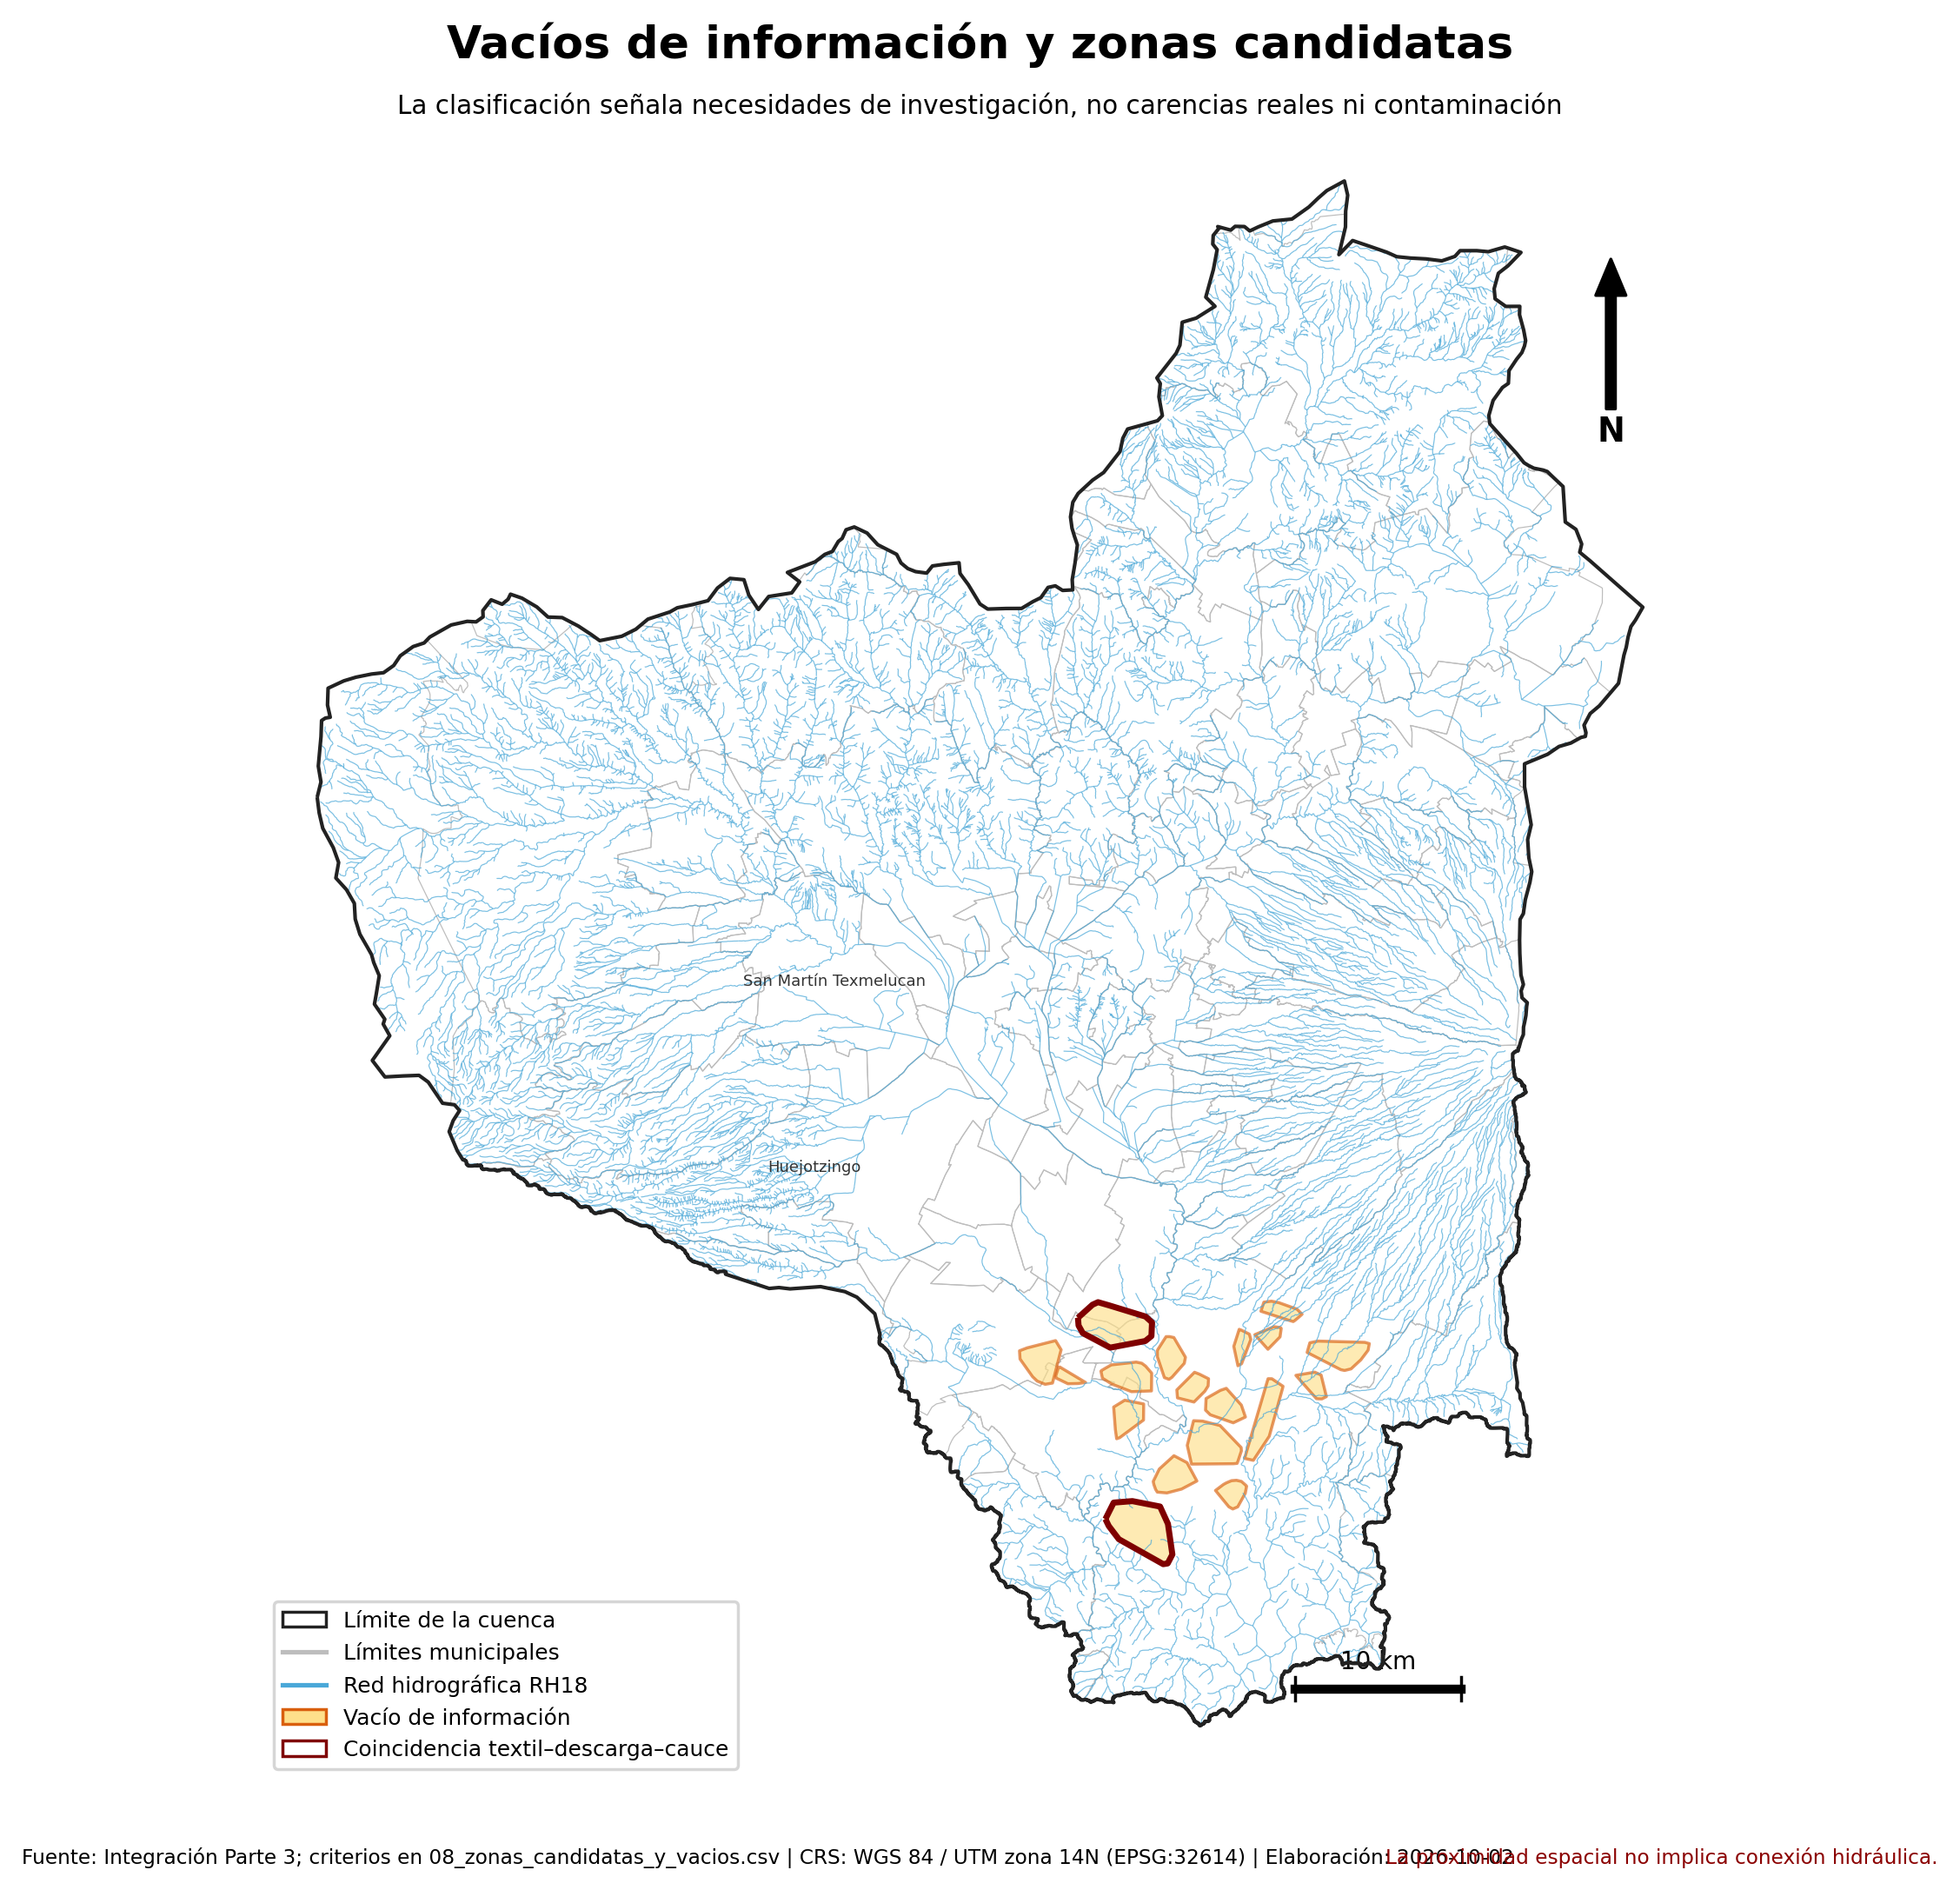
\includegraphics[width=.88\textwidth]{09_vacios_y_zonas_candidatas.png}\caption{Vacíos de información y coincidencias candidatas para investigación posterior.}\label{fig:vacios}\end{figure}

\pregunta{P9. ¿Qué se observa en Huejotzingo frente a San Martín Texmelucan?}
\metodo{Se recortaron establecimientos, PTAR, descargas e hidrografía con cada polígono municipal.}
\begin{table}[H]\centering\small\caption{Comparación registral de los municipios de interés.}\begin{tabular}{lrr}
\toprule Indicador & Huejotzingo & San Martín Texmelucan\\\midrule
Establecimientos & 450 & 460\\
Alta relevancia & 14 & 10\\
PTAR registradas (incluye posibles duplicados) & 4 & 2\\
Capacidad con dato (L/s) & 85 & 190\\
Caudal tratado con dato (L/s) & 38 & 100\\
Descargas registradas & 1 & 1\\
Trazos de colector recuperables & 0 & 0\\\bottomrule
\end{tabular}\end{table}
\resultado{Los municipios tienen cantidades semejantes de establecimientos, pero la información de capacidad se distribuye de forma distinta. Huejotzingo presenta dos plantas con capacidad reportada; San Martín, una de mayor capacidad nominal. Las Figuras~\ref{fig:huejo} y \ref{fig:smt} muestran diferencias internas en distribución territorial.}
\limite{Las diferencias reflejan simultáneamente infraestructura y disponibilidad de datos; no permiten concluir cuál municipio tiene mejor cobertura.}
\begin{figure}[H]\centering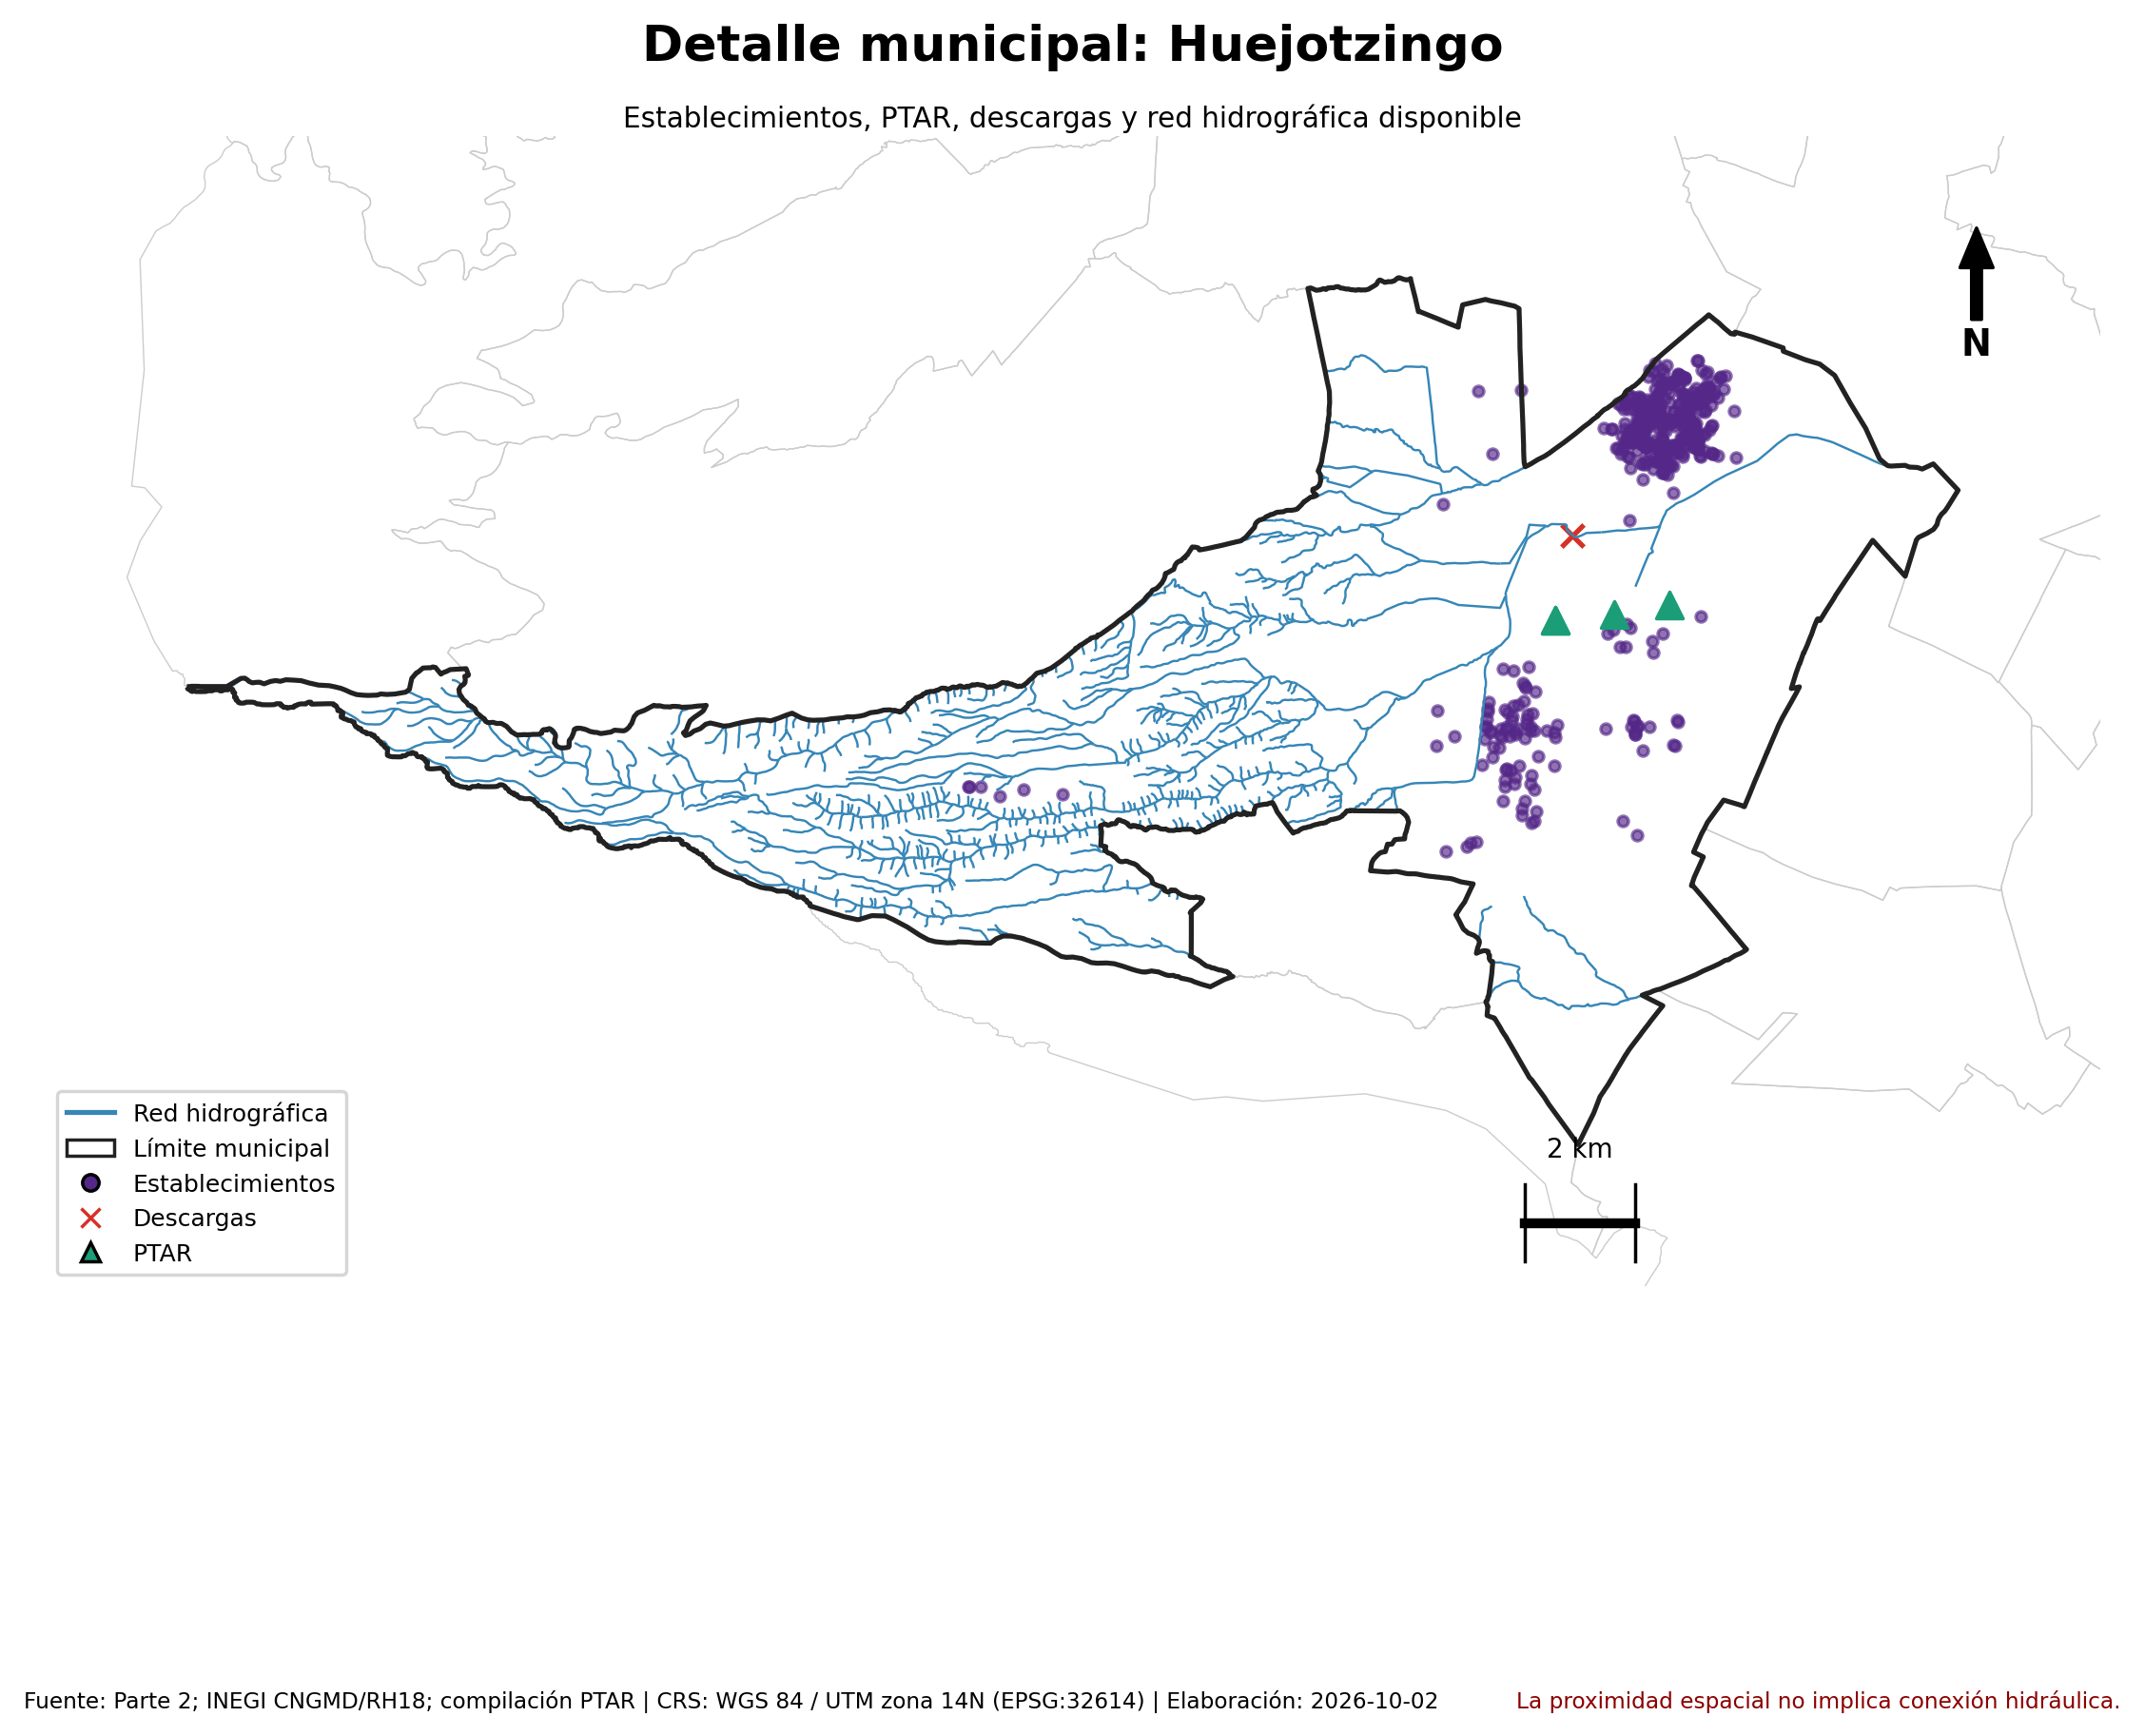
\includegraphics[width=.9\textwidth]{07_detalle_huejotzingo.png}\caption{Detalle de Huejotzingo.}\label{fig:huejo}\end{figure}
\begin{figure}[H]\centering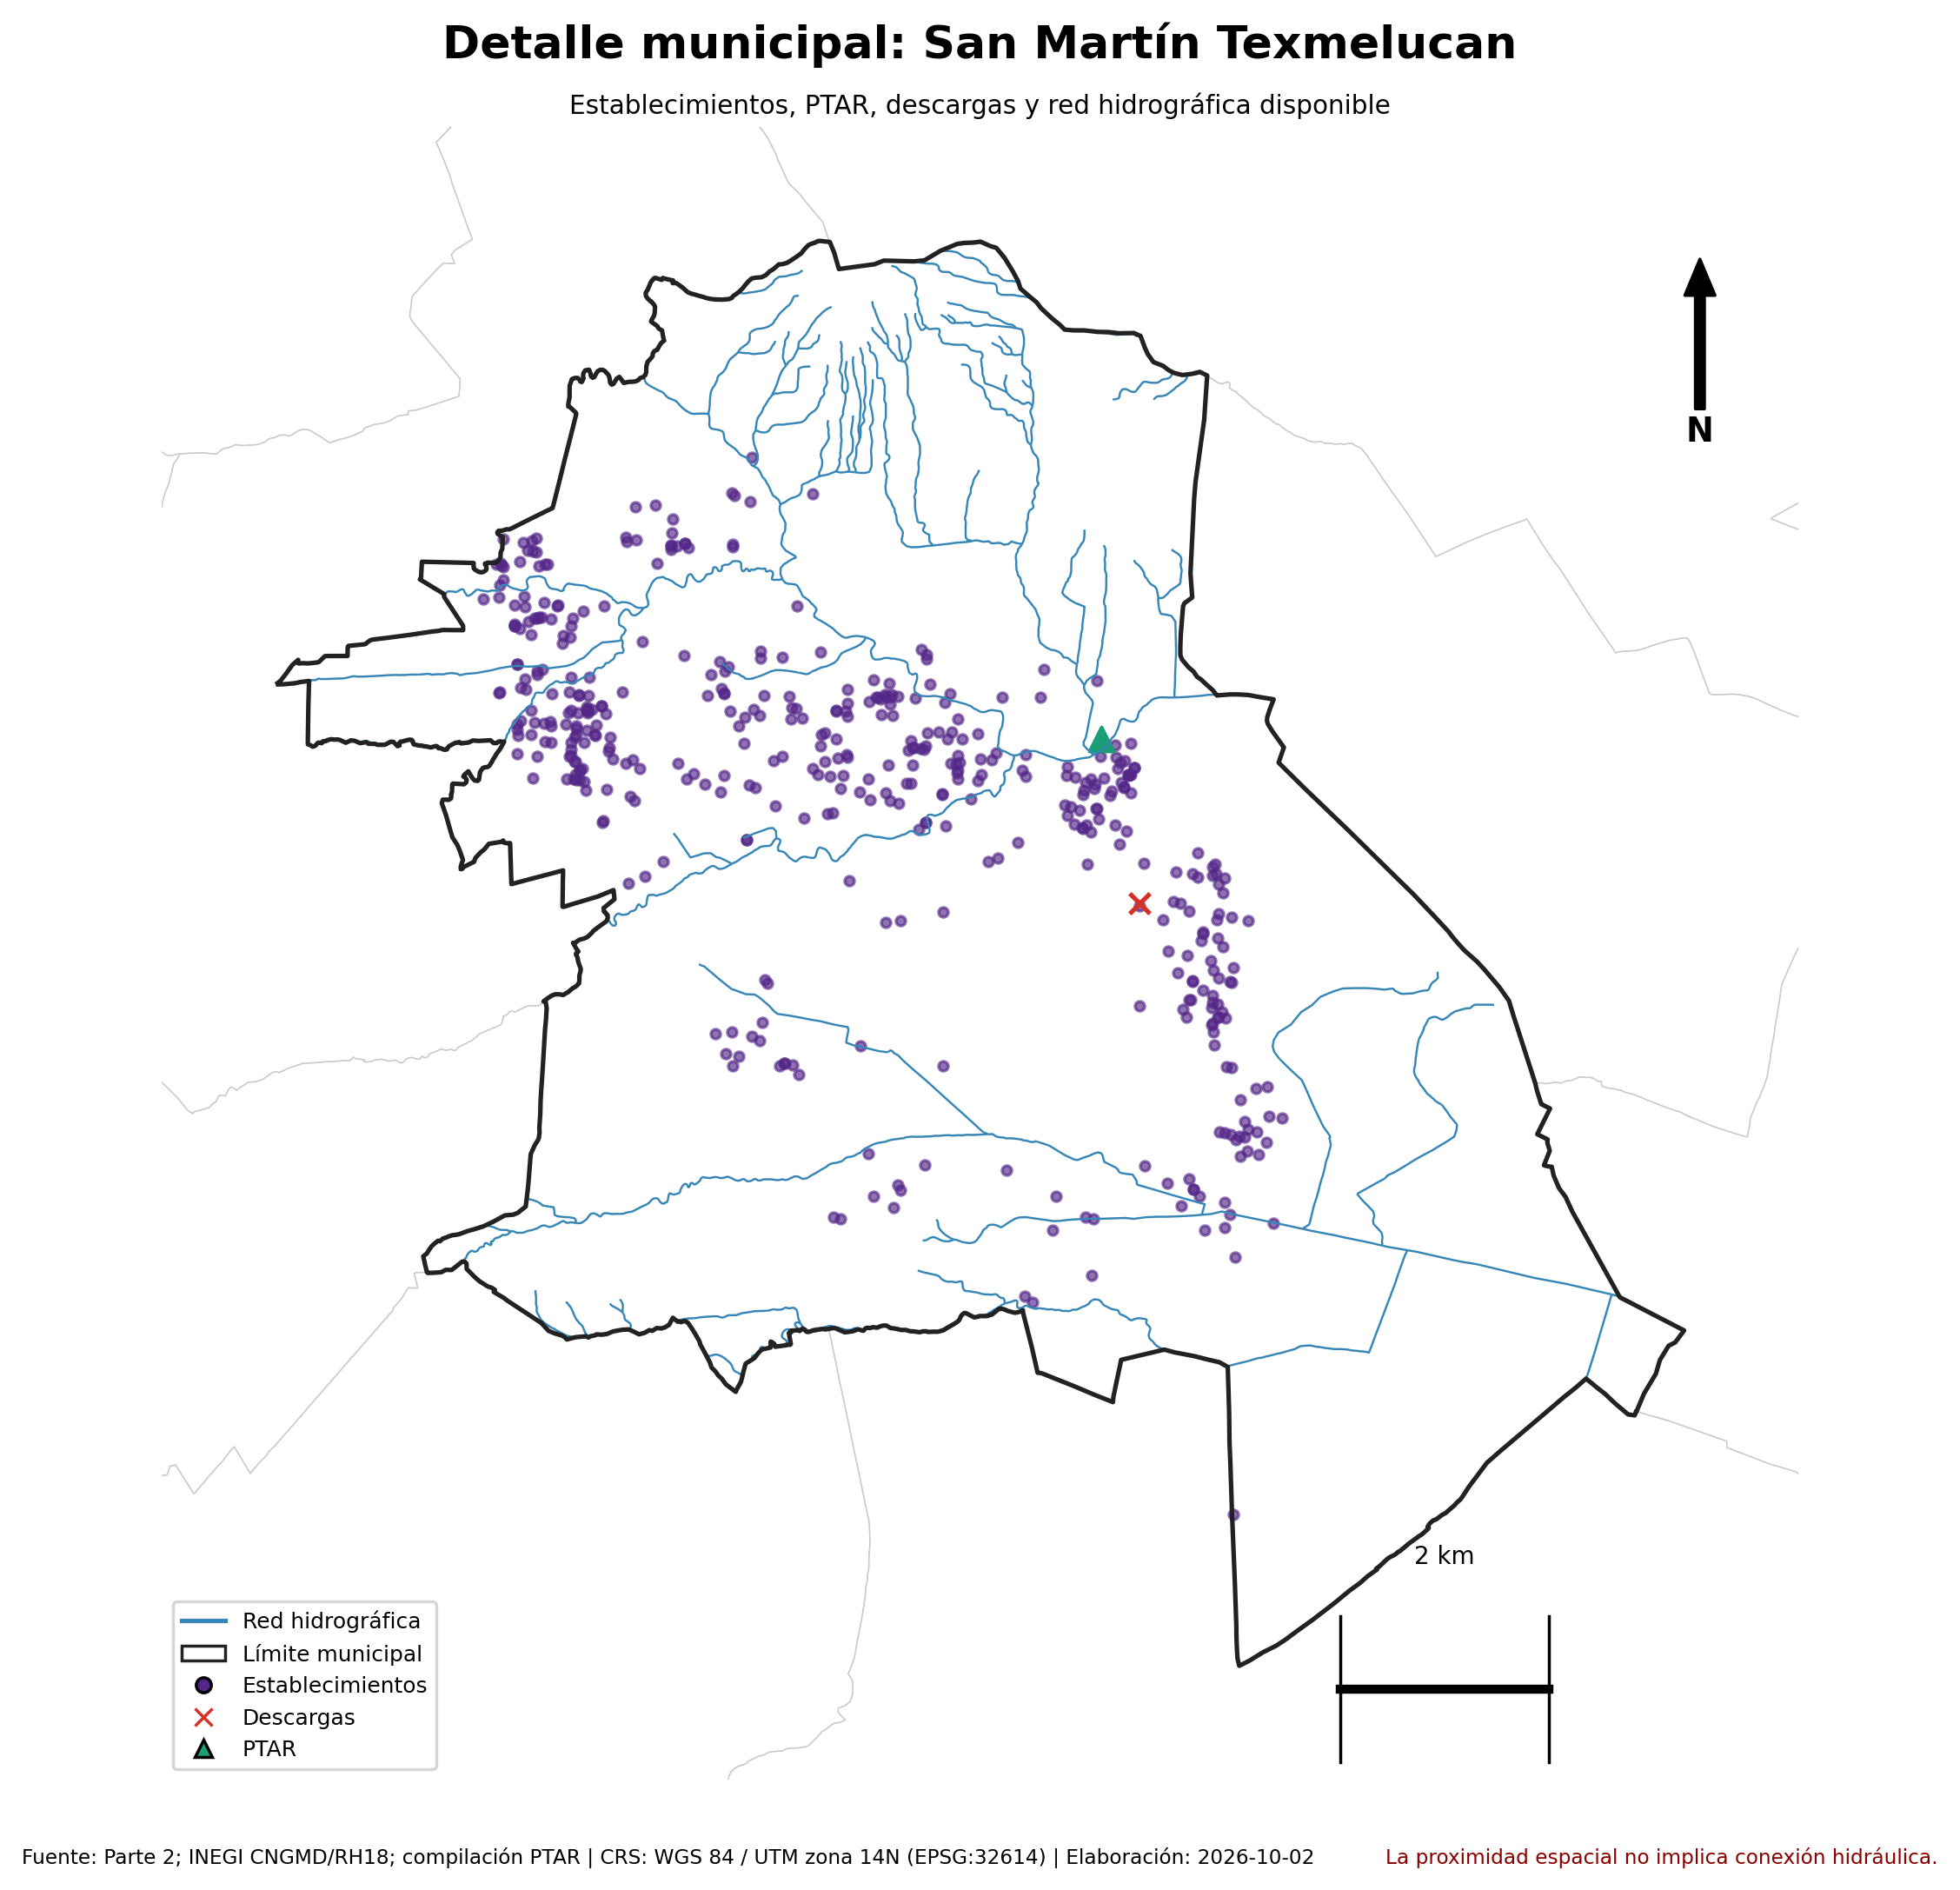
\includegraphics[width=.9\textwidth]{08_detalle_san_martín_texmelucan.png}\caption{Detalle de San Martín Texmelucan.}\label{fig:smt}\end{figure}

\pregunta{P10. ¿Qué relaciones están documentadas y cuáles son plausibles?}
\begin{table}[H]\centering\small\caption{Matriz sintética de evidencia.}\begin{tabular}{p{3cm}p{3cm}cp{7cm}}\toprule Origen&Destino&Nivel&Fundamento\\\midrule
Establecimiento&Colector&D&Sin geometría ni vínculo documental recuperable\\
Establecimiento&Descarga&C&Proximidad euclidiana únicamente\\
Establecimiento&PTAR&C&Proximidad euclidiana únicamente\\
Colector&Descarga/PTAR&D&No existe capa recuperable de colectores\\
Descarga&Cuerpo receptor&A/C&A si la fuente declara receptor; C si sólo es el cauce próximo\\
PTAR&Cuerpo receptor&A/D&A si está declarado; D si falta el atributo\\
Subnúcleo&Infraestructura&C&Coincidencia territorial agregada\\\bottomrule\end{tabular}\end{table}
\resultado{Ninguna cadena completa establecimiento--colector--descarga/PTAR--receptor queda documentada de extremo a extremo. La matriz es una guía para solicitar evidencia y diseñar trabajo de campo.}

\section{Síntesis: rutas potencialmente asociadas con la actividad textil}
\subsection*{A. Evidencia disponible}
Se conocen localizaciones de establecimientos, concentraciones territoriales, PTAR y descargas registradas, además de la red hidrográfica superficial y algunos atributos de capacidad, caudal, proceso y receptor.
\subsection*{B. Inferencias espaciales plausibles}
Pueden identificarse elementos cercanos, subnúcleos con coincidencia territorial y cauces próximos. SUB\_04 y SUB\_05 justifican investigación posterior por la simultaneidad de señales, no por evidencia de contaminación.
\subsection*{C. Información faltante}
Faltan red de alcantarillado, colectores verificables, sentido y capacidad de conducciones, áreas de servicio, estado operativo de PTAR, caudales de descarga, permisos vigentes, elevación y vínculos documentales entre usuarios e infraestructura.
\subsection*{D. Datos por obtener}
Se deben solicitar planos \emph{as-built}, catastro de drenaje, permisos y títulos de descarga, bitácoras de operación, capacidad efectiva, polígonos de servicio y monitoreo de caudal/calidad. En campo deben validarse trazos, dirección, accesos, puntos de descarga y condiciones operativas.
\subsection*{E. Análisis ya habilitados}
Son válidos los análisis de proximidad, vacíos de información, coincidencia territorial, comparación registral municipal, conciliación de fuentes y priorización preliminar de verificación.
\subsection*{F. Análisis que todavía no deben hacerse}
No debe reconstruirse una ruta hidráulica completa, asignarse una descarga o PTAR a un establecimiento, estimarse carga contaminante, afirmarse cobertura/suficiencia ni proponerse causalidad sin los datos faltantes.

\section{Conclusiones}
La Parte 3 produce una base común y auditable, no un modelo hidráulico terminado. Su principal resultado es hacer explícito qué está observado, qué es proximidad y dónde faltan datos. La siguiente etapa debe integrar relieve y drenaje sanitario con evidencia operativa, y usar las zonas candidatas para dirigir solicitudes de información y validación de campo.

\appendix
\section{Productos reproducibles}
Las tablas completas se encuentran en \texttt{outputs/parte\_3/06\_analisis/}; el diccionario, trazabilidad, conciliación de PTAR y control de calidad están en \texttt{outputs/parte\_3/}. Los scripts \texttt{302\_integrar\_sistema\_saneamiento\_parte3.py} y \texttt{303\_analisis\_y\_mapas\_parte3.py} regeneran la integración y el análisis.
\end{document}
